%%
%% This is file `sample-authordraft.tex',
%% generated with the docstrip utility.
%%
%% The original source files were:
%%
%% samples.dtx  (with options: `authordraft')
%% 
%% IMPORTANT NOTICE:
%% 
%% For the copyright see the source file.
%% 
%% Any modified versions of this file must be renamed
%% with new filenames distinct from sample-authordraft.tex.
%% 
%% For distribution of the original source see the terms
%% for copying and modification in the file samples.dtx.
%% 
%% This generated file may be distributed as long as the
%% original source files, as listed above, are part of the
%% same distribution. (The sources need not necessarily be
%% in the same archive or directory.)
%%
%% The first command in your LaTeX source must be the \documentclass command.
\documentclass[sigchi,authordraft]{acmart}

%% 追加
\usepackage{bm}
\newcommand\figref[1]{\textbf{Figure~\ref{fig:#1}}}
\newcommand\tabref[1]{\textbf{Table~\ref{tab:#1}}}
\usepackage{url}
\usepackage{color}
%% ここまで

%%%% As of March 2017, [siggraph] is no longer used. Please use sigconf (above) for SIGGRAPH conferences.

%%%% As of May 2020, [sigchi] and [sigchi-a] are no longer used. Please use sigconf (above) for SIGCHI conferences.

%%%% Proceedings format for SIGPLAN conferences 
% \documentclass[sigplan, anonymous, authordraft]{acmart}

%%%% Proceedings format for conferences using one-column small layout
% \documentclass[acmsmall,authordraft]{acmart}

% NOTE that a single column version is required for submission and peer review. This can be done by changing the \doucmentclass[...]{acmart} in this template to 
% \documentclass[manuscript,screen]{acmart}

%%
%% \BibTeX command to typeset BibTeX logo in the docs
\AtBeginDocument{%
  \providecommand\BibTeX{{%
    \normalfont B\kern-0.5em{\scshape i\kern-0.25em b}\kern-0.8em\TeX}}}

%% Rights management information.  This information is sent to you
%% when you complete the rights form.  These commands have SAMPLE
%% values in them; it is your responsibility as an author to replace
%% the commands and values with those provided to you when you
%% complete the rights form.
\setcopyright{acmcopyright}
\copyrightyear{2020}
\acmYear{2020}
\acmDOI{10.1145/1122445.1122456}

%% These commands are for a PROCEEDINGS abstract or paper.
% \acmConference[Woodstock '18]{Woodstock '18: ACM Symposium on Neural
%   Gaze Detection}{June 03--05, 2018}{Woodstock, NY}
% \acmBooktitle{Woodstock '18: ACM Symposium on Neural Gaze Detection,
%   June 03--05, 2018, Woodstock, NY}
% \acmPrice{15.00}
% \acmISBN{978-1-4503-XXXX-X/18/06}


%%
%% Submission ID.
%% Use this when submitting an article to a sponsored event. You'll
%% receive a unique submission ID from the organizers
%% of the event, and this ID should be used as the parameter to this command.
%%\acmSubmissionID{123-A56-BU3}

%%
%% The majority of ACM publications use numbered citations and
%% references.  The command \citestyle{authoryear} switches to the
%% "author year" style.
%%
%% If you are preparing content for an event
%% sponsored by ACM SIGGRAPH, you must use the "author year" style of
%% citations and references.
%% Uncommenting
%% the next command will enable that style.
%%\citestyle{acmauthoryear}

%%
%% end of the preamble, start of the body of the document source.
\begin{document}

%%
%% The "title" command has an optional parameter,
%% allowing the author to define a "short title" to be used in page headers.
\title{User Identification Method based on Head Shape\\using a Helmet with Pressure Sensors}

%%
%% The "author" command and its associated commands are used to define
%% the authors and their affiliations.
%% Of note is the shared affiliation of the first two authors, and the
%% "authornote" and "authornotemark" commands
%% used to denote shared contribution to the research.
\author{Atsuhiro Fujii}
\affiliation{%
  \institution{Ritsumeikan University}
  \city{Shiga}
  \country{Japan}}
\email{atsuhiro.fujii@iis.ise.ritsumei.ac.jp}

\author{Kazuya Murao}
\affiliation{%
  \institution{Ritsumeikan University}
  \city{Shiga}
  \country{Japan}}
\email{murao@cs.ritsumei.ac.jp}

%%
%% By default, the full list of authors will be used in the page
%% headers. Often, this list is too long, and will overlap
%% other information printed in the page headers. This command allows
%% the author to define a more concise list
%% of authors' names for this purpose.
\renewcommand{\shortauthors}{Fujii and Murao}

%%
%% The abstract is a short summary of the work to be presented in the
%% article.
\begin{abstract}
Helmets are used for various purposes such as industrial protective hat (work helmet), motorcycle Helmet, sports helmet, and military/police helmet. If the wearer is known through wearing a shared helmet, name, affiliation, qualification can be shown on a display mounted on the helmet, and sensor data collected through helmet such as acceleration data, video, eye track data can be labeled with wearer's ID.
%It can also be used as a door key in factories when access to the room is restricted by job title or other reasons.
In this paper, we propose a user identification method based on User's head shape using a helmet equipped with 32 pressure sensors. Our method has two functions: identification and authentication. Identification is to classify users into one of the registered users. Authentication is to accept users who have been registered to the system and reject unknown users. We have implemented a prototype helmet device and collected data from nine subjects, resulting in 100\% accuracy for user identification and 0.076 average EER for user authentication.

%ヘルメットは社会生活において広く利用されている.本研究では32個の圧力センサを搭載したヘルメットを装着することで,頭部形状から個人を識別する手法を提案する.提案手法によって,ヘルメット上部に取り付けたディスプレイに名前を表示したり,視線情報などのデータを記録する際に手間なく作業者のラベルを付与できる.また,工場などで役職などにより入室できる部屋が制限されている場合に扉の鍵としても使用できる.提案手法は,あらかじめデータが登録された複数の人物のうちの1人がヘルメットを装着したときにその人物を識別する個人識別と,ヘルメットを装着した人物が登録者であれば認証し,登録者でなければ拒否する本人認証の2つの機構を備える.プロトタイプデバイスと解析用のソフトウェアを実装した後,被験者9人データを採取し,個人識別では精度が100\%,本人認証では被験者全員の平均EERが約7.6\%という結果を得た.
\end{abstract}

%%
%% The code below is generated by the tool at http://dl.acm.org/ccs.cfm.
%% Please copy and paste the code instead of the example below.
%%
\begin{CCSXML}
<ccs2012>
 <concept>
  <concept_id>10010520.10010553.10010562</concept_id>
  <concept_desc>Computer systems organization~Embedded systems</concept_desc>
  <concept_significance>500</concept_significance>
 </concept>
 <concept>
  <concept_id>10010520.10010575.10010755</concept_id>
  <concept_desc>Computer systems organization~Redundancy</concept_desc>
  <concept_significance>300</concept_significance>
 </concept>
 <concept>
  <concept_id>10010520.10010553.10010554</concept_id>
  <concept_desc>Computer systems organization~Robotics</concept_desc>
  <concept_significance>100</concept_significance>
 </concept>
 <concept>
  <concept_id>10003033.10003083.10003095</concept_id>
  <concept_desc>Networks~Network reliability</concept_desc>
  <concept_significance>100</concept_significance>
 </concept>
</ccs2012>
\end{CCSXML}

\ccsdesc[500]{Computer systems organization~Embedded systems}
\ccsdesc[300]{Computer systems organization~Redundancy}
\ccsdesc{Computer systems organization~Robotics}
\ccsdesc[100]{Networks~Network reliability}

%%
%% Keywords. The author(s) should pick words that accurately describe
%% the work being presented. Separate the keywords with commas.
\keywords{User identification, pressure sensor, helmet, head shape}

%% A "teaser" image appears between the author and affiliation
%% information and the body of the document, and typically spans the
%% page.
% \begin{teaserfigure}
%   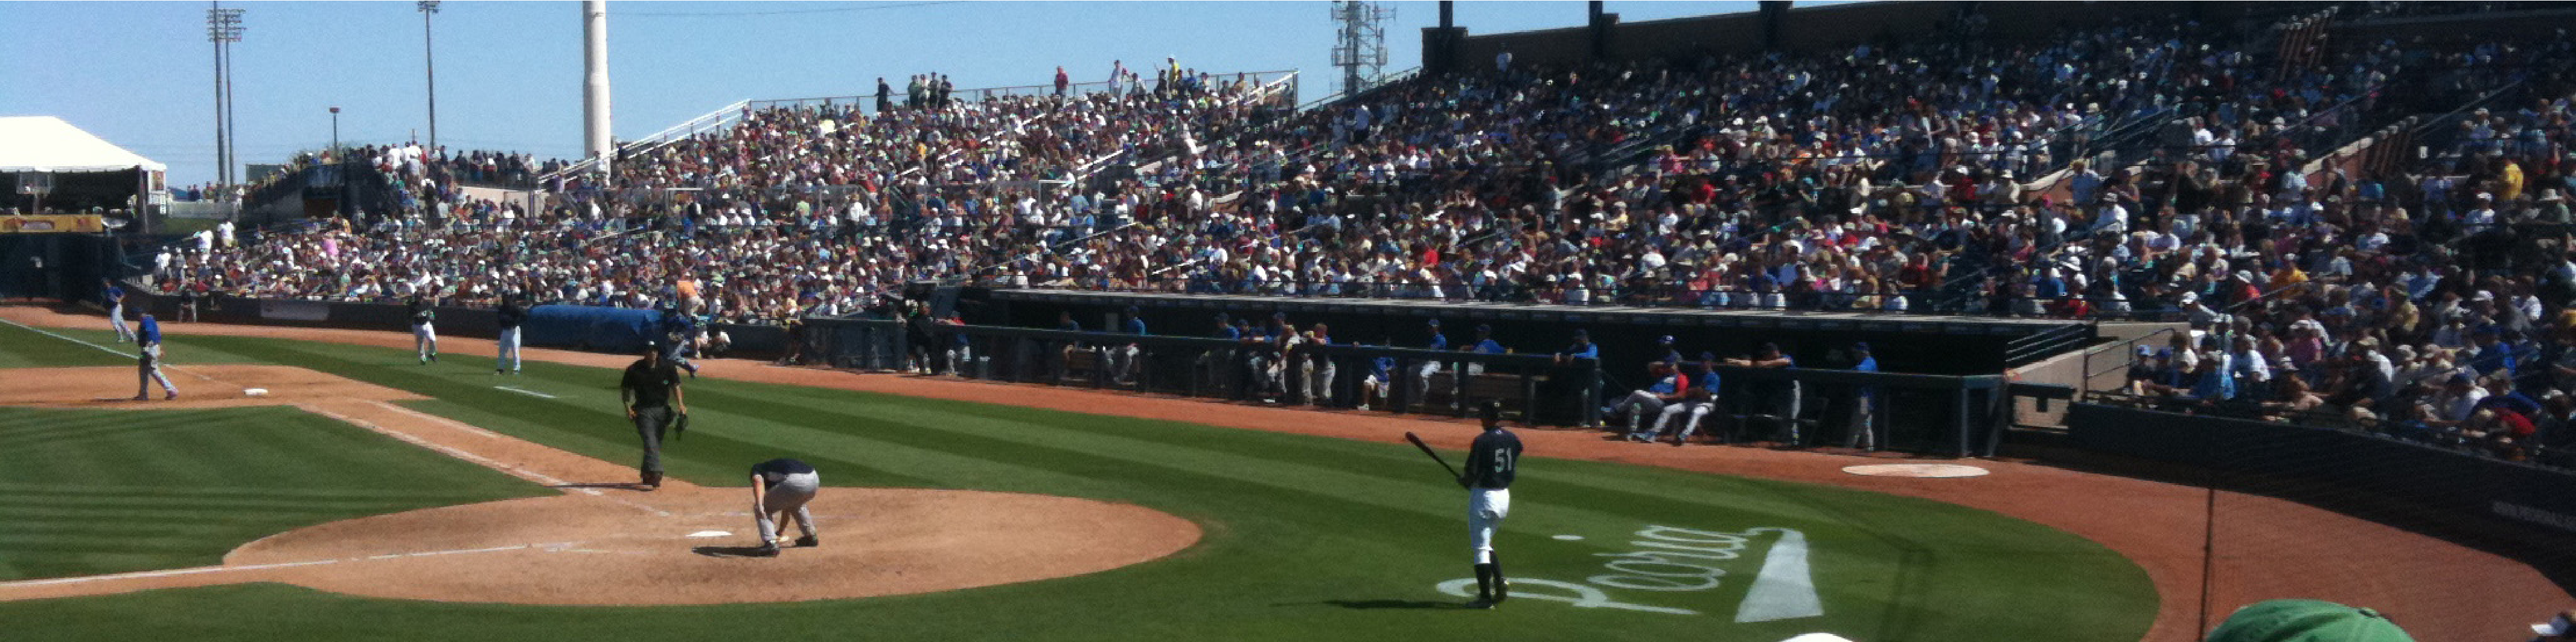
\includegraphics[width=\textwidth]{sampleteaser}
%   \caption{Seattle Mariners at Spring Training, 2010.}
%   \Description{Enjoying the baseball game from the third-base
%   seats. Ichiro Suzuki preparing to bat.}
%   \label{fig:teaser}
% \end{teaserfigure}

%%
%% This command processes the author and affiliation and title
%% information and builds the first part of the formatted document.
\maketitle

\section{Introduction}
\label{sec:introduction}
Helmets are used for various purposes such as industrial protective hat (work helmet), motorcycle Helmet (bike, car, bicycle, etc.), sports helmet (American football, baseball, ice hokey, etc.), and military/police helmet. These are all worn to protect the head in the event of an accident\cite{helmet}. It is considered important from a safety point of view that there is no gap between the head and the helmet.\par

%ヘルメットは,スポーツやレジャー,バイク乗車時,工場,災害現場など,社会生活において広く利用されている.これらはいずれも,事故発生時に頭部を保護する目的で着用\cite{helmet}するものであり,頭部との隙間がないことが安全面において重要だとされている.\par

Workers in factories and disaster sites have to wear helmets. There are also various people who do not know each other, such as short-term workers and vendors. If these people have own helmet, the wearer's name and work division are shown on the helmet, allowing the helmet wearer to be identified from a distance or overhead even if the wearer's face cannot clearly be seen. Identifying individuals is a deterrent to trespassers. In addition, showing the qualifications such as a hazardous materials engineer's license and heavy machinery licence helps create a safe work environment. In many cases, such information is directly written on the helmet or an identifiable sticker is attached to the helmet. However, in such an analog operation, it is easy for a trespasser to disguise himself by writing or stealing a sticker. Moreover, even if the worker puts on other people's helmet, they are not aware of it and wrong information is displayed. If the helmets are shared among the workers, the helmet is not marked with the identifiable information.\par
%「貸与されたヘルメットの場合,ヘルメットに名前が表示されておらず,現場にいる者どうしも誰であるかを判断できず,不審者が容易に侵入できる可能性がある.」は,書いてない時点で不審者なのでは?と突っ込まれる.実際は,ペンで書いたりシール貼るアナログな方式だと不審者が簡単に偽装できるのが問題かな.問題は3つあって,シールや直書きでは1)不審者による偽装2)取り間違え,共用の場合は情報が表示されない.

%特に,工場や災害現場ではほぼ全員がヘルメットを装着して作業し,短期労働者や業者など,互いに顔を知らないさまざまな人間が出入りしている.一人1個のヘルメットを所有している場合はヘルメットに氏名がテープ等で表示されていため,ヘルメットを装着したままでも遠くからあるいは頭上からでも識別できる.また,作業者によって所持している資格や従事可能な作業が異なるため,所有資格を示すステッカーが販売されており,そのような作業者のヘルメットに貼り付けて識別できるようにしている.しかし,貸与されたヘルメットの場合,ヘルメットに名前が表示されておらず,現場にいる者どうしも誰であるかを判断できず,不審者が容易に侵入できる可能性がある.また,仮に名前が表示されていたとしても,取り間違いによって,作業者とヘルメットの氏名が異なる場合もある.\par

In this paper, we propose a method that identifies users based on the shape of their heads by installing pressure sensors inside a helmet. We implemented a prototype helmet with 32 pressure sensors. Our method calculates the similarity between the wear's data and registered users' data and outputs the user of the most similar data as an identification result.\par
%本研究ではヘルメットの内部に圧力センサを搭載することで,頭部形状から個人を識別する手法を提案する.

The prototype helmet has a display to show user's name and credentials upon the identification result, therefore, wrong information is not displayed on the helmet if a helmet of someone else is used. It is useful that the identification information is automatically displayed on a shared helmet and workers can recognize each other. In addition, another advantage of user identification is data annotation. Data collected through sensors attached to the helmet or wears' body such as a camera, an eye tracker, and an accelerometer can automatically be annotated with the wear's ID. By attaching a GPS module or an antenna to localize the user\cite{disaster_en}, the name and location of the worker can be determined in real time and it will be easier for the foreman to understand the overall situation in the field. Furthermore, from the pressure data between the helmet and the head, it is possible to check whether the shape of the head matches the helmet as zero pressure value means that there is a gap between the helmet and the head.
%提案手法によって,ヘルメット上部に取り付けたディスプレイに名前や資格情報を表示できるため,ヘルメットが共用でも互いに認識でき,取り違えることもない.また,ヘルメットに取り付けられたカメラや視線計測装置,各種センサのデータを自動で作業者と紐づけることができる.さらに,GPSモジュールとアンテナ\cite{disaster_en}を取り付けることで,リアルタイムに作業員の名前と位置情報を送信することができれば,現場の全体の状況が把握しやすくなる.さらには,頭部形状を取得することによりヘルメットと頭部の隙間や圧迫の情報を取得できるため,ヘルメットと頭部形状が合っているかを確認することもできる.\par
Another possible use of the proposed helmet is a key for the door where access to the room is restricted according to the position or qualifications. \par
%It can also be used for a key of motorcycle. Using the helmet for identification instead of physical key, the risk of key theft and key lost is reduced.\par


The proposed method has two functions: user identification and user authentication. User identification is based on the assumption that a single helmet is shared by several people. The pressure sensor data of a person who may wear a helmet is registered in advance, and the person who wears the helmet is identified as one of the registered persons. Personal identification does not assume that a non-registered person will wear the device. If a non-registered person wears the device, the identification result will be the one with the closest data among the registered users.
The user authentication determines whether the person wearing the helmet is actually the person with the ID or not when the ID of a user wearing a helmet is given to the system. We assume an environment in which each individual has own helmet (the same as for smartphone authentication) and an environment in which the user ID is entered when using a shared helmet (the same as for ATM authentication). Even if an outsider wears a helmet and enters the stolen ID, they can be identified as an outsider (authentication denied) because their head shape is different from the person of the ID.
%提案手法は個人識別と個人認証の2種類の機能をもつ.個人識別は1つのヘルメットを複数人で共有する場面を想定している.装着する可能性のある人の圧力センサのデータを事前に登録しておき,装着したときに登録者のうちの誰であるかを識別する.個人識別では,登録されていない人が装着することは想定しておらず,仮に登録されていない人が装着した場合は,登録者のうち最もデータが近い人が識別結果となる.
%個人認証はヘルメットを装着するユーザのIDが与えられたときに,実際に装着している人がそのIDの人物であるか否かを判定する.個人ごとに専用のヘルメットが用意されている環境(スマートフォンの認証と同じ)や,共有のヘルメットを使用時にユーザIDを入力する環境(ATMの認証と同じ)が想定される.部外者が装着して盗み取ったIDを入力しても,頭部形状が異なるため部外者として識別(認証拒否)できる.

%このほか,工場などで役職や資格により入室できる部屋が制限されている場合の扉の鍵としての使用や,バイクの鍵としても使用できる.ヘルメットでの本人識別を行うため,鍵の盗難による侵入,車両盗難のリスクの減少にも繋がる.\par



%行動的特徴を使うアプローチの場合,ヘルメットを装着する時点で個人が識別されている必要があるため,ヘルメットを被る動作を特徴とすることも考えられる.筆者らはこれまでにスマートフォンをポケットから取り出す際の加速度センサデータから認証する手法\cite{murao_screen_unlock}を提案した.スマートフォンはポケットや机の上など取る場面が限定されるが,ヘルメットを取る場面は様々であり,この手法をヘルメットに適用することは困難であると考えられる.\par

In the following sections, Section \ref{sec:related} introduces the related works, Section \ref{sec:method} explains the proposed method, Section \ref{sec:evaluation} evaluates the proposed method, and Section \ref{sec:conclusion} concludes this paper.

%以降本稿では,\ref{related}節で関連研究を紹介する.\ref{method}節で提案手法を説明し,\ref{evaluation}節で提案手法の評価実験と結果の考察を行い,最後に\ref{conclude}節で本研究をまとめる.

\section{Related Work}
\label{sec:related}
In this section, we introduce research on user identification and head state recognition.

% 本節では個人認証手法,身体部位装着型デバイス,頭部状態の認識に関する研究を紹介する.

\subsection{User Authentication Method}
%%%%%%%%%%%%%ほかの認証手法のはなし
There are several methods to identify individuals: password, PIN, and stroke pattern; physical characteristics such as face, fingerprint, voice print, and iris; and behavioral characteristics such as handwriting and gait. Password, PIN, and stroke pattern that can be freely set by individuals has a risk of spoofing by shoulder hacking, brute force attack, and password duplication.\par

%個人を識別する手法として,パスワードやPIN,ストロークパターンなどの本人がカギを自由に設定できる手法,顔,指紋や筆跡,声紋,光彩などの身体的特徴を用いる手法,筆跡や歩容などの行動的特徴を用いる手法がある.個人が自由に設定できるパスワードやPIN,ストロークパターンのみを用いて,本研究で想定するような多数の人間の識別を行うことは,パスワードの重複や総当たり攻撃によるなりすましの危険性がある.\par

For physical characteristics, Chen et al.\cite{face_and_finger} proposed an authentication method using the user's face and fingertips video images captured from the front and rear cameras of a mobile device. It is possible to identify the wearer by using a camera mounted on the helmet, however, it is messy to take a picture of the face all the time wearing the helmet. 
Siddharth et al.\cite{palm_print} proposed an authentication system based on palm print and palm vein. The system uses visible and infrared light to acquire images of the palm print and palm vein, and the authentication is performed by checking the data against the registration data in the database. 
Sayo et al.\cite{lip_motion} proposed an authentication method based on the camera image capturing the shape of the lips which is a physical characteristics and the movement of the lips during speech which is behavioral characteristics. 
As another method using the mouth, Kim et al.\cite{teeth_and_voice} proposed an authentication method that combines dental images and voice. Bednarik et al.\cite{eye_movement} proposed an identification system that uses eye movements such as pupil size and variation, gaze velocity, and distance of the infrared reflection of the eye. 

For such camera-based approaches, mounting a camera on the outside of the helmet, individuals can be identified by turning toward the camera before putting on the helmet. However, there is a complication of taking a picture of one's own face with a camera. For the method using palm print and palm vein, this method also requires the user to hold the camera each time the wearing the helmet. A camera can be attached to the mouth of the helmet so that the shape and movement of the lips and teeth can be acquired. However, the space around the mouth inside the full-face helmet is limited, and it is difficult to distinguish the shape and movement of around the mouth with a single camera. In addition, it is not practical as helmets have to be considered being used in the dark places.

%指紋認証
Nogueira et al.\cite{finger_CNN} used convolutional neural networks (CNN) for fingerprint authentication, and achieved a high classification accuracy. However, fingerprint authentication has a risk that fingerprints can be easily duplicated from photographs. The head shape we use in this paper is a physical characteristic, and is difficult to be replicated because of its three-dimensional shape.\par

%Nogueiraら\cite{finger_CNN}は,畳み込みニューラルネットワーク(CNN)を用いて指紋認証を行うことで,高い分類精度を実現している.しかし,指紋は写真などから容易に複製できるリスクがある.


%身体的特徴に関して,Chenら\cite{face_and_finger}はスマートフォンなどの端末のフロントカメラとリアカメラから得られる顔と指先のビデオ映像からユーザ本人を認証する手法を提案している.ヘルメットの外部にあらかじめカメラを取り付けておくことで装着者を識別できると考えられるが,暗所や雨天では認識精度が低下する恐れがある.また,毎回ヘルメットを被る前に,ヘルメットを持って自身の顔を撮影することは面倒である.指紋認証\cite{finger_CNN}は,指紋が写真などから容易に複製されるリスクがある.本研究で用いた頭部形状は,個人ごとに身体的特徴を持つ.また,立体形状であるため複製が困難であると考える.\par

For behavioral characteristics, it may be possible to authenticate the users by focusing on the action of wearing a helmet. The authors have proposed a method that authenticates a smartphone user from acceleration sensor data when taking it out of the pocket\cite{murao_screen_unlock}. Guerra-Casanova et al.\cite{accelerometer_authentification} proposed a method to authenticate users by gestures of their hands using a mobile device with an embedded accelerometer. For motion-based authentication using accelerometers, there is a possibility that the acceleration characteristics of the motion until the helmet is worn can be used for authentication by mounting an accelerometer on the helmet. However, there are various wearing actions, such as wearing the helmet in a hurry and taking care not to let the interior of the helmet get wet in the rain. Therefore, it is not practical to collect data from all the people in various situations.\par

%Bednarikら\cite{eye_movement}は,瞳孔の大きさと変化,視線速度,目の赤外線反射の距離などの眼球運動を使用した生体認証を提案した.Chenら\cite{face_and_finger}はモバイルデバイスのフロントカメラとリアカメラで顔と指先のビデオ映像を同時に撮影し,個別の映像から抽出された2つのフォトプレチスモグラムを比較することにより,その一貫性から認証を行う手法を提案している.Siddharthら\cite{palm_print}は掌紋と掌静脈を用いた生体認証システムを提案している.このシステムでは,可視光線と赤外線を使用して掌紋と掌静脈の画像を取得し,データベース内の登録データと照合することで認証を行っている.Sayoら\cite{lip_motion}は,身体的特徴である口唇の形状と,行動的特徴である発話に伴う口唇の動きをカメラで撮影して認証する手法を提案した.また,口元を用いた他の手法として,Kimら\cite{teeth_and_voice}は歯の画像と音声を組み合わせた認証手法を提案している.\par


%このようなカメラを使用したアプローチの場合,カメラをヘルメットの外側に取り付けておけば,ヘルメットを装着する前にカメラの方を向くことで個人を識別できるが,わざわざカメラで自身の顔を撮影する煩雑さがある.掌紋と掌静脈での認証の場合はヘルメットの側頭部にカメラを取り付け,着用時に握ることで実装が可能であるが,こちらの手法も装着するたびカメラを握らなければならない.フルフェイス型ヘルメットであれば,ヘルメットの口元にカメラを取り付けることで,口唇の形状,動きや歯の画像を取得できるが,ヘルメット内部の口元の空間は限られるため,口とカメラの距離が近くなってしまい,1個のカメラで口唇の形状や動きを判別することは困難である.また,すべてのヘルメットにカメラを装着する手間や経済的な問題がある.悪天候による水没や暗所での使用も考慮しなければならず,現実的ではない.\par

%ヘルメットでのジェスチャ認証

%加速度センサを用いたジェスチャ認証の場合,ヘルメットに加速度センサを搭載することで,ヘルメットを装着するまでの動作の加速度の特徴量を用いて認証できる可能性がある.しかしながら,急いでいて動作が速くなる場合や,雨天時にヘルメットの内装が濡れないように気をつけながら装着する場合など,ヘルメットを装着する動作は多様であり,さまざまな状況において装着する可能性のある人全員のデータを採取して学習しておくことは現実的ではない.\par



% \subsection{Body Part Mounted Devices}
% %デバイスとしての新規性
% Ham et al.\cite{smart_wristband} proposed a wristband device as an input device for smart glasses. This device has a touch screen panel (TSP) and inertial measurement unit (IMU), and it is manipulated by touching and the twisting of your wrist. Since the device can be worn on the wrist, the user is not restricted in his or her movements and has a high degree of freedom of movement. In addition, a touch panel is used for pointing to improve the stability of input. Hernandez et al.\cite{bioglass} proposed a method for recognizing pulse and respiration rates from accelerometers, gyroscopes, and cameras embedded in Google Glass, a head-worn wearable device. Nishajith et al.\cite{smart_cap} designed and implemented a head-worn wearable device which is named smart cap for assist visually impaired people with situational awareness. This devices are consists of Raspberry Pi 3, Raspberry Pi NoIR Camera V2, and an earpiece and power supply. Raspberry Pi NoIR (No Infrared)  Camera V2 is an infrared camera module for Raspberry Pi. An audio description of the object detected in the image obtained from this infrared camera is given through the earpiece.\par

% %Hamら\cite{smart_wristband}はスマートグラス用の入力デバイスとして,リストバンド型のデバイスを提案している.このデバイスはタッチパネルと慣性計測ユニットを搭載しており,タッチや手首をひねるなどのモーションで操作ができる.手首にデバイスを装着することで使用できるため,ユーザは動きを制限されず,自由度が高い.また,ポインティングにはタッチパネルを使用することで,入力の安定性を向上させた.Hernandezら\cite{bioglass}は頭部装着型のウェアラブルデバイスである,Google Glassに内蔵された加速度センサ,ジャイロセンサ,カメラから脈拍数と呼吸数を認識する手法を提案している.Nishajithら\cite{smart_cap}は,視覚障害者の状況認識を支援するウェアラブルデバイスとして,スマートキャップの設計と実装を行った.デバイスはRaspberry Pi 3,Raspberry Pi NoIR Camera V2,イヤホン,電源から構成される.Raspberry Pi NoIR(No Infrared) Camera V2とはRaspberry Piの赤外線カメラモジュールである.この赤外線カメラで得られる画像から検出された対象物について,イヤホンを通して音声で説明する.\par

% These are all studies on wearable devices worn on body parts, and the shape of device is varied. Head-worn wearable devices such as cap and eyeglass exist, but there are no studies using helmets to the best of our knowledge.

% %これらはいずれも身体部位に装着するウェアラブルデバイスに関する研究であり,さまざまな形状のデバイスを用いた研究が行われている.特に,頭部装着型のウェアラブルデバイスとしては帽子型や眼鏡型などが存在するが,ヘルメットを用いた研究は筆者らの知る限り存在しない.

\subsection{Head State Recognition}
%頭部形状を認識するという点での新規性
Toth et al.\cite{facial_expression_headset} focused on the facial muscle signal, and six different facial expressions were classified using the muscle signals and the gyroscope values which were got from a cheap off-the-shelf electroencephalogram (EEG) headset. EEG headsets are actually used to measure brain waves, however, the muscle signals are detected locally since the measurement is performed by placing electrodes on the scalp. It uses only existing EEG devices for classification of facial expressions and no additional electromyography (EMG) sensor is used.
Kwon et al.\cite{facial_expression_glasses} designed a glass-type wearable device to detect the user's emotions based on facial expressions and physiological reactions. The device can capture facial expressions with a built-in camera and obtain physiological responses such as photoplethysmogram (PPG) and electrodermal activity (EDA).
Fukumoto et al.\cite{fukumoto} designed a smile-based life-logging system that focuses on smile/laughter for indexing the interesting/enjoyable events on a recorded video. They use photo-interrupters and smile/laughter is detected separately by threshold-based clustering. Evaluation results showed 73\%--94\% accuracy in detecting smile/laughter while actual use of the system.
%Electroencephalogram(EEG)ヘッドセットは脳波の計測に用いられるが,頭皮に電極を配置して計測を行うため,局所的に筋信号が検出される.多くの場合はノイズとして除去されるが,Tothら\cite{facial_expression_headset}はこの筋信号に注目し,安価なElectroencephalogram(EEG)ヘッドセットから得られる筋信号とジャイロセンサの値を用いて,6種類の表情の分類を行った.表情の分類に既存の脳波デバイスを使用することで,別途追加で筋電位(EMG)センサを用意する必要がなくなり,よりハイブリッドな脳コンピュータインタフェース(BCI)システムを構築できる.Kwonら\cite{facial_expression_glasses}は顔の表情と生理反応を利用して,利用者の感情を検出するメガネ型ウェアラブルデバイスを設計している.設計したデバイスは,内蔵したカメラで顔の表情が取得できる.また,フォトプレチスモグラム(PPG)や皮膚電気活動(EDA)などの生理的反応を取得できる.これらを用いて利用者の感情を検出する.\par
%福本さんの笑顔のやつも入れる.フォトリフレクタで表情認識もあるはず.
These researches obtain dynamic information such as facial expressions and physical responses in the face area. On the other hand, our study differs from them in that it obtains static features of the head shape.\par

Kouno et al.\cite{head_top_camera} proposed an image-based person identification system using an depth image from an overhead camera. By using depth information, this system captures the precise person’s area and four features extracted from images based on depth information to the identification method; body height, body dimensions, body size and depth histogram. The identification accuracy is 94.4\% and 91.4\% while standing in front of a door and touching a doorknob, respectively.
%これらの研究は,表情や顔部分の身体的反応などの動的な情報を取得するものであり,対して本研究は静的な頭部形状の特徴を取得するという点で異なる.\par

In this paper, we propose a method to identify individuals by acquiring their head shape while wearing a helmet with pressure sensors. Our method does not force the users to do special behavior or to remain stationary for identification. Taking a wearable approach, our method can be used in any place and any time. To breach the system, the exact three-dimensional shape of the head is needed, but it is difficult to replicate the head shape.

%本研究では内装に圧力センサを搭載したヘルメットを装着することで,頭部形状を取得して個人識別する手法を提案する.提案手法は個人識別のために特別な動作を必要とせず,デバイスの搭載によって動作が制限されることもない.さらに,認証に用いる頭部形状を複製するには立体形状を正確に把握する必要があり,複製が困難である.

\section{Proposed Method}
\label{sec:method}
This section describes the details of the proposed method.

%本節では提案手法の詳細を述べる.

\subsection{Overview}
The proposed method assumes that the user wears a helmet equipped with pressure sensors, acquires the shape of wearer's head, and identifies whether the wearer is registered person or not. The proposed method has two functions: user identification and user authentication.
\begin{itemize}
    \item {\bf User identification} assumes that a single helmet is shared by multiple people and any other information such as ID is not given to the system; users just wear the helmet. Their pressure sensor data are registered in advance and the person who put on the helmet is identified as one of the registered persons as shown in \figref{system_classification}. User identification does not assume that a non-registered person will wear the helmet. If a non-registered person wears the device, the identification result will be the one with the closest data among the registered users.
    
    \item {\bf User authentication} determines whether the person wearing the helmet is actually the person or not when his/her ID or username is given. We assume two cases where the authentication is used: each individual has own helmet and only the person's pressure sensor data has been registered (single user; username preset in the device; the same as for smartphone authentication); and a helmet is shared with multiple people and username is entered when using the helmet (multiple users; username input accordingly; the same as for ATM authentication). Their pressure sensor data are registered in advance and the person who put on the helmet is judged to be accepted or rejected by calculating the similarity between the input data and the data of the ID as shown in \figref{system_mahalanobis}. Even if an ID is leaked, an outsider can be rejected because his/her head shape is different from the data of the ID.
\end{itemize}

%提案手法は,利用者が圧力センサを搭載したヘルメットを装着することで,頭部形状を取得し,装着者が事前に登録された人物であるかを識別する.本研究では2つの利用環境を想定する.一つ目は\figref{system_classification}に示すように,複数の人物が登録されており,登録された人物(登録者)のうちのいずれかがヘルメットを装着した際に,その人物が登録者のうち誰かを認識する環境である.二つ目は,\figref{system_mahalanobis}に示すように,1人以上の人物が登録されており,登録された人物以外を含む人物がヘルメットを装着した際に,その人物が登録者であれば認証し,登録者でなければ拒否する環境である.前者の環境を個人識別,後者の環境を本人認証と呼ぶ.

32 pressure sensors are attached to the inner side of the helmet to acquire data, producing 1-dimensional 32-channel pressure data. Pressure data of the people who are expected to wear helmets have been registered to the system in advance and the data is called training data in this paper. In user identification, the system uses the Support Vector Machine (SVM) to build a recognition model from the feature values extracted from the training data and outputs the identification results from the features of the input data of an unknown registrant in the identification phase. On the other hand, in user authentication, the system calculates Mahalanobis' distance between the training data and the input data of the person including non-registrant is calculated and authenticates the user if the distance is less than the threshold, otherwise the user is rejected.

%ヘルメットの内側には32個の圧力センサが搭載されており,32次元のデータを取得する.提案システムでは,業務などでヘルメットを装着すると想定される人物を登録者として事前にヘルメットを装着してもらい,圧力センサデータを学習データとして収集しておく.個人識別では,識別したい利用者全員にヘルメットを複数回装着してもらうことで頭部の32次元の圧力センサデータ群を収集し,Support Vector Machine(SVM)を用いて学習データから認識モデルを構築しておく.そして,識別フェーズで未知の登録者の入力データの特徴から識別結果を求める.一方,本人認証では,認証したい利用者にヘルメットを複数回装着してもらうことで頭部の32次元の圧力センサデータ群を収集しておく.そして,識別フェーズで登録者以外も含む人物の入力データと学習データ群とのマハラノビス距離を計算し,距離が閾値以下であれば本人であるとして認証する.

\begin{figure}[!t]
  \centering
    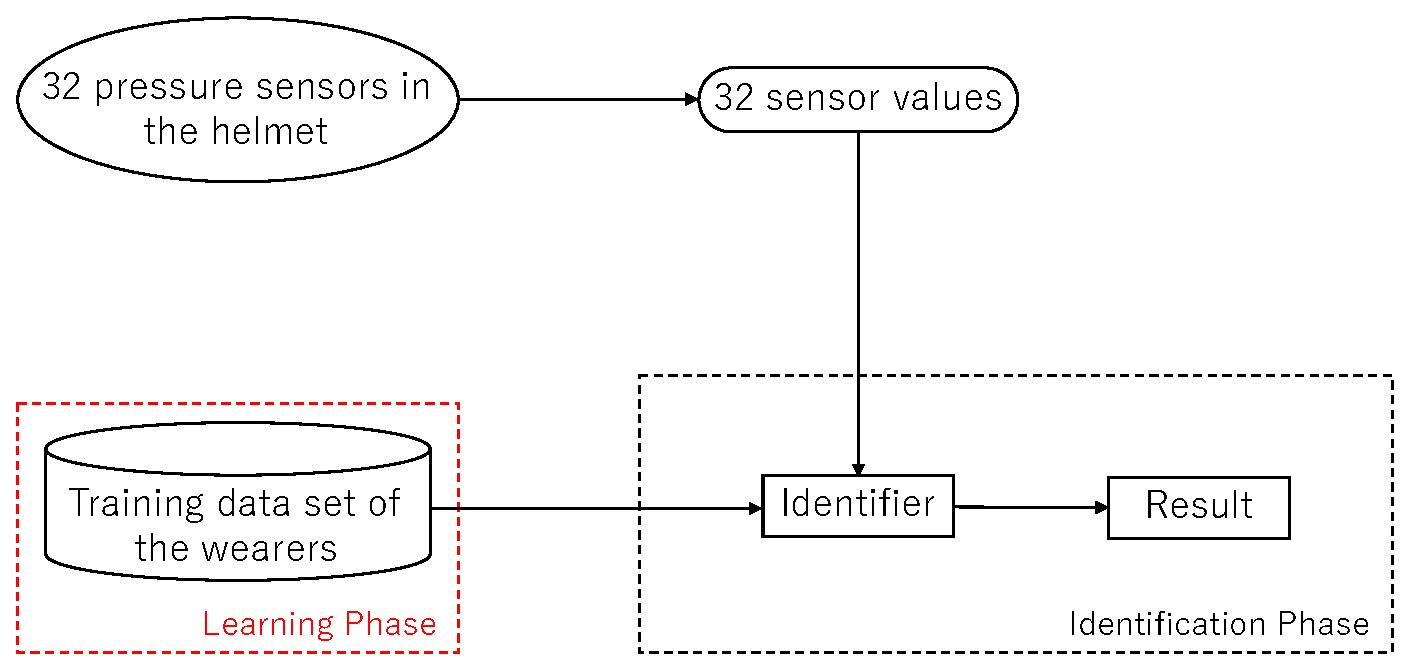
\includegraphics[width=1\linewidth]{figure/system_classification.eps}
  \caption{Structure of the user identification.}
  \label{fig:system_classification}
\end{figure}

\begin{figure}[!t]
  \centering
    \includegraphics[width=1\linewidth]{figure/system_mahalanobis.eps}
  \caption{Structure of the user authentication.}
  \label{fig:system_mahalanobis}
\end{figure}

\subsection{Hardware}
We implemented a helmet equipped with 32 pressure sensors. \figref{device} shows the configuration of the device and \figref{met_over} shows the appearance of the device.
%提案手法に用いる圧力センサを搭載したヘルメットを実装した.デバイスの構成を\figref{device}に,デバイスの外観を\figref{met_over}に示す.\par
The head of the helmet wearer must be in close contact with the sensors to obtain the correct pressure values, therefore, we used a commercially available full-face helmet with high adhesion. The pressure sensors were FSR402 and FSR402 ShortTail manufactured by Interlink Electronics, Inc. The Arduino MEGA2560 R3 was used as a microcomputer. Since the helmets used were free size and it was difficult to attach and remove the interior, we removed the interior of the top of the head and installed a thick urethane sponge as shown in \figref{met_in}. The urethane sponge is cut and a pressure sensor was inserted into the cut line as shown in \figref{sensor}. 

Four pressure sensors were set at the top of the head, 16 sensors were set around the top of the head, six sensors were set at the back of the head, and six sensors were set at the cheek pads on both sides. A total of 32 sensors were installed at the points as shown in \figref{position}. The wiring for the pressure sensors went through a hole drilled in the top of the helmet, then it is connected to 5V power supply port, GND, and analog input port which is on the Arduino MEGA2560 R3 via a printed circuit board (PCB) with a 10 K$\Omega$ resistor which is mounted outside the helmet. The PCB attached to the outside of the helmet is shown in \figref{print}. The PCB is bolted to the left cheek area using a threaded hole drilled for securing the helmet shield. It is fixed and removable.

%圧力値を正しく取得するには,センサとヘルメット装着者の頭部が密着している必要があるため,密着度の高いフルフェイス型ヘルメット(B\&B社製BB100)を用いた.圧力センサとしてインターリンクエレクトロニクス社製のFSR402およびFSR402 ShortTailを合計32個使用した.マイコンとしてArduino MEGA2560 R3を使用した.使用したヘルメットはフリーサイズであり,内装の脱着が困難であったため,\figref{met_in}に示すように頭頂部の内装を取り外して,新たに厚みのあるウレタンスポンジを取り付けた.また,\figref{sensor}に示すようにウレタンスポンジの中央部に切り込みを入れて圧力センサを挿し込んだ.圧力センサは頭頂部に4個,頭頂部周囲に16個,後頭部に6個,左右チークパッド部に6個の合計32個を搭載した.この位置を\figref{position}に示す.配線はヘルメットの頭頂部にドリルで開けた穴から,ヘルメット外部に取り付けた10K$\Omega$の抵抗を配線してあるプリント基板を経由して,Arduino MEGA2560 R3の5V電源,GND,アナログ入力ポートに接続した.ヘルメット外部に取り付けたプリント基板を\figref{print}に示す.プリント基板はヘルメットのシールド固定用に開けられたネジ穴を用いて左頬部分にボルトで固定しており,取り外しが可能である.

\begin{figure}[!t]
  \begin{center}
    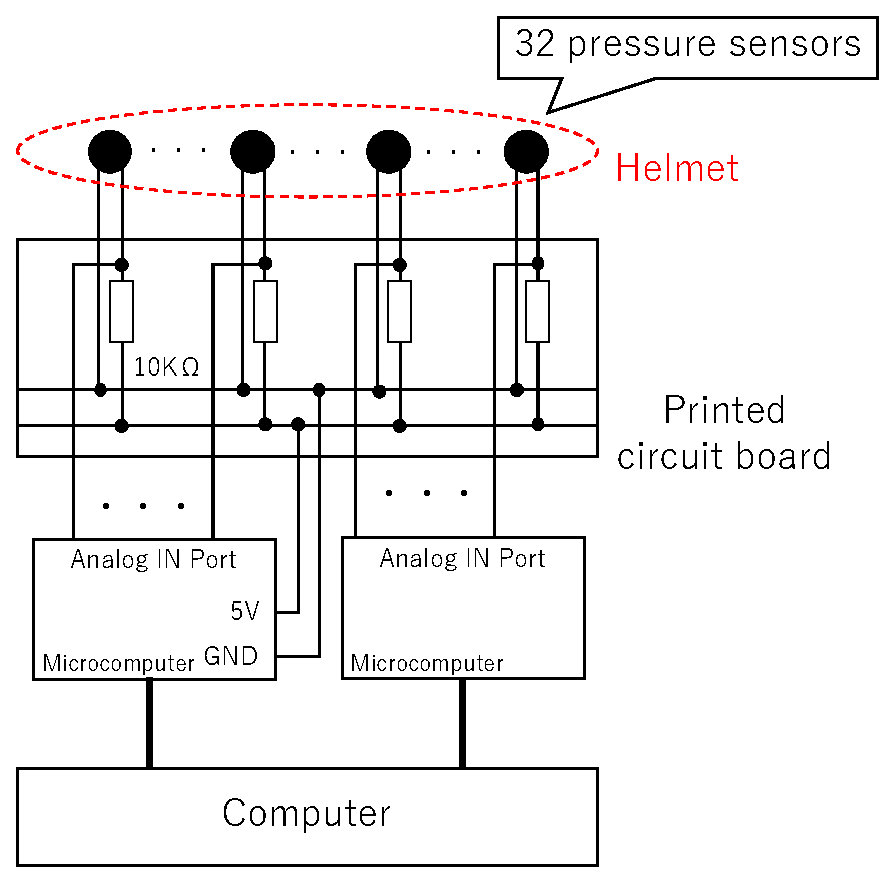
\includegraphics[width=0.5\linewidth]{figure/device.eps}
  \end{center}
  \caption{Structure of the device}
  \label{fig:device}
\end{figure}

\begin{figure}[!t]
  \begin{center}
    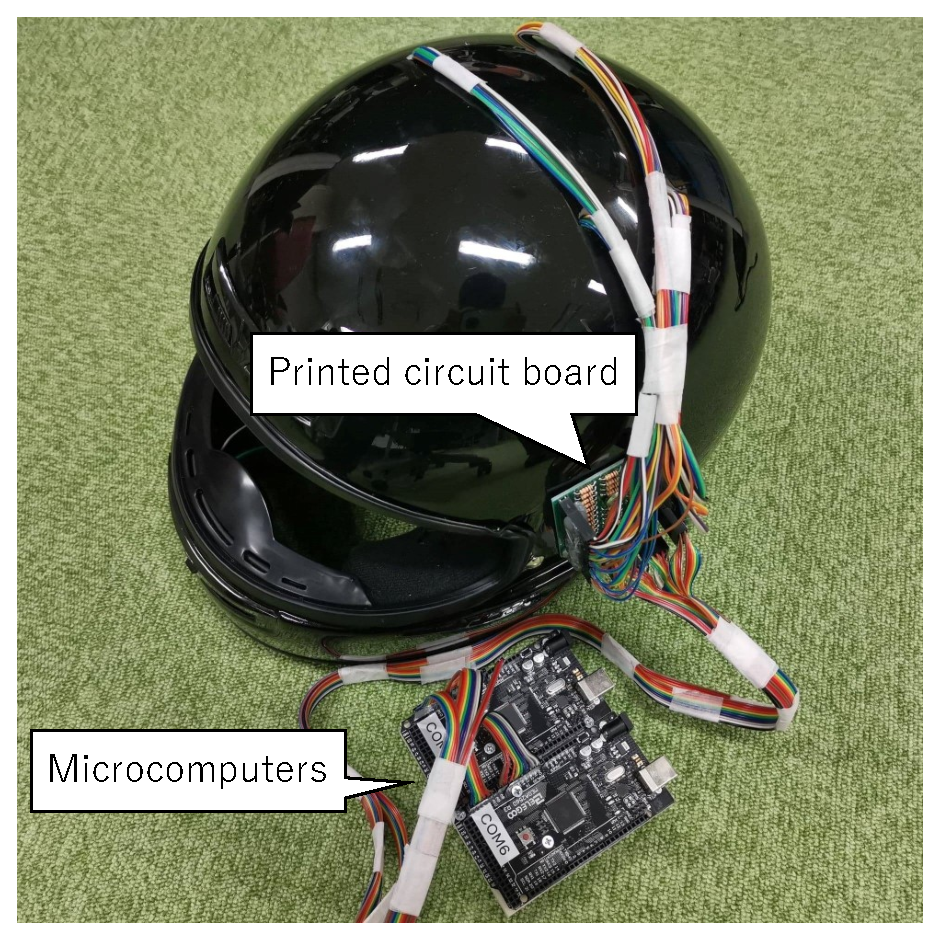
\includegraphics[width=0.4\linewidth]{figure/met_over.eps}
  \end{center}
  \caption{Appearance of the device}
  \label{fig:met_over}
\end{figure}

\begin{figure}[!t]
  \begin{center}
    \includegraphics[width=0.6\linewidth]{figure/met_in.eps}
  \end{center}
  \caption{Inside of the device}
  \label{fig:met_in}
\end{figure}

\begin{figure}[!t]
  \begin{center}
    \includegraphics[width=0.6\linewidth]{figure/sensor.eps}
  \end{center}
  \caption{Mounting Method for Pressure Sensors}
  \label{fig:sensor}
\end{figure}

\begin{figure}[!t]
  \begin{center}
    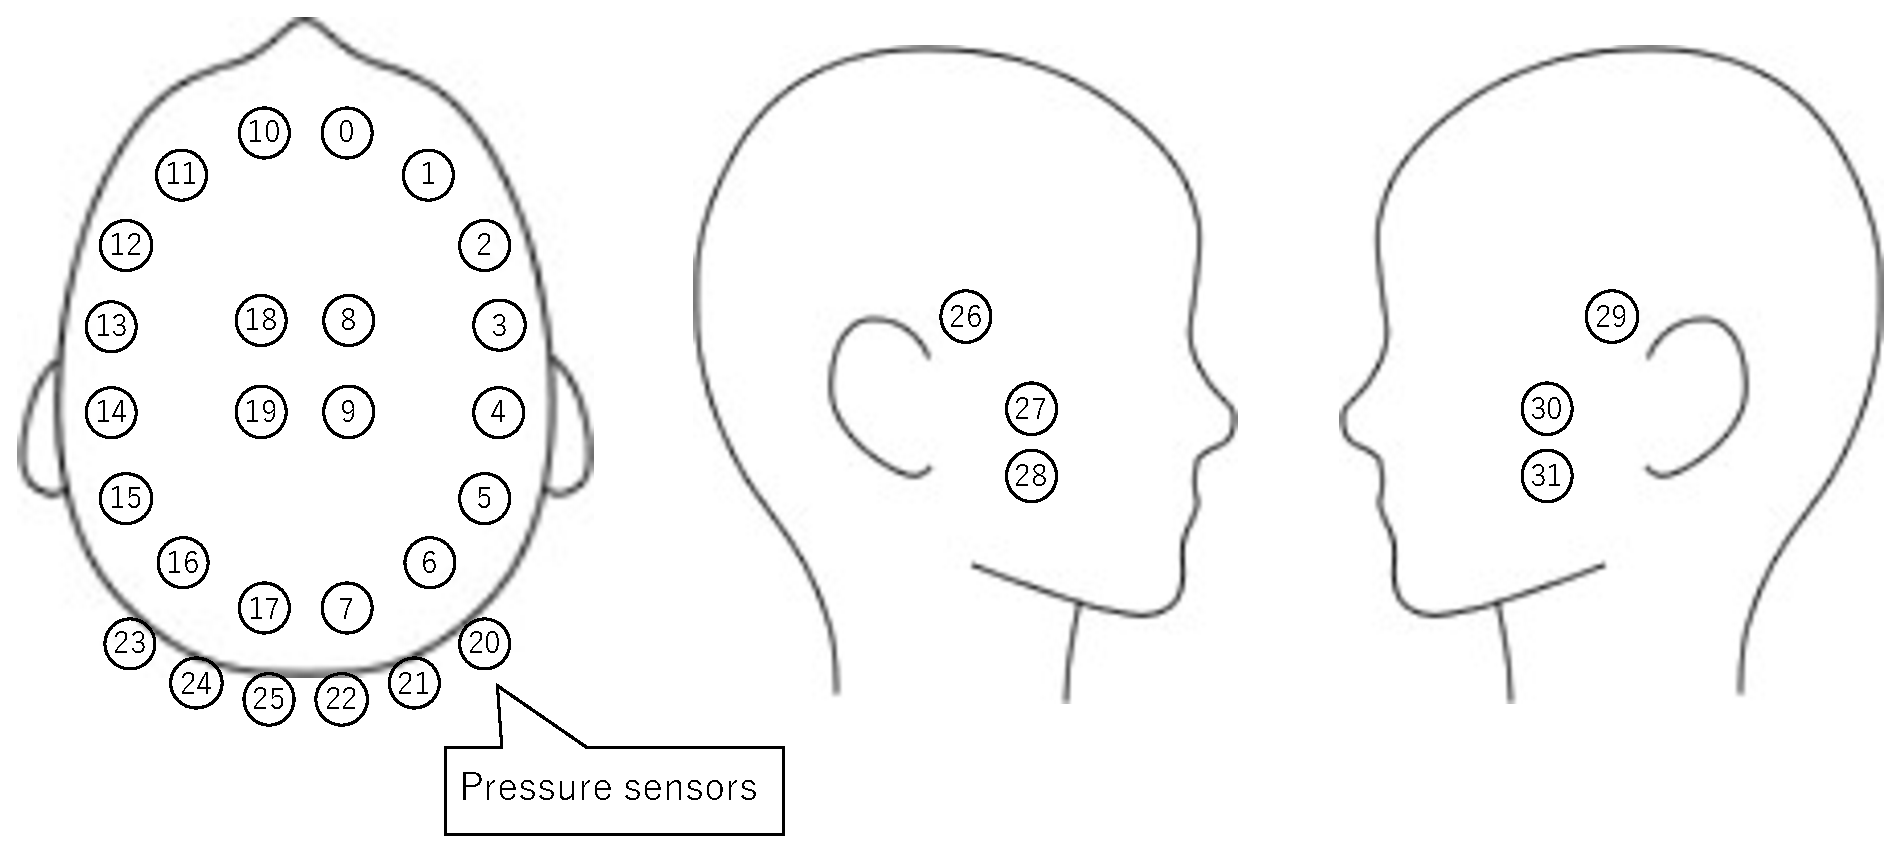
\includegraphics[width=1\linewidth]{figure/position.eps}
  \end{center}
  \caption{The position of the pressure sensors}
  \label{fig:position}
\end{figure}

\begin{figure}[!t]
  \begin{center}
    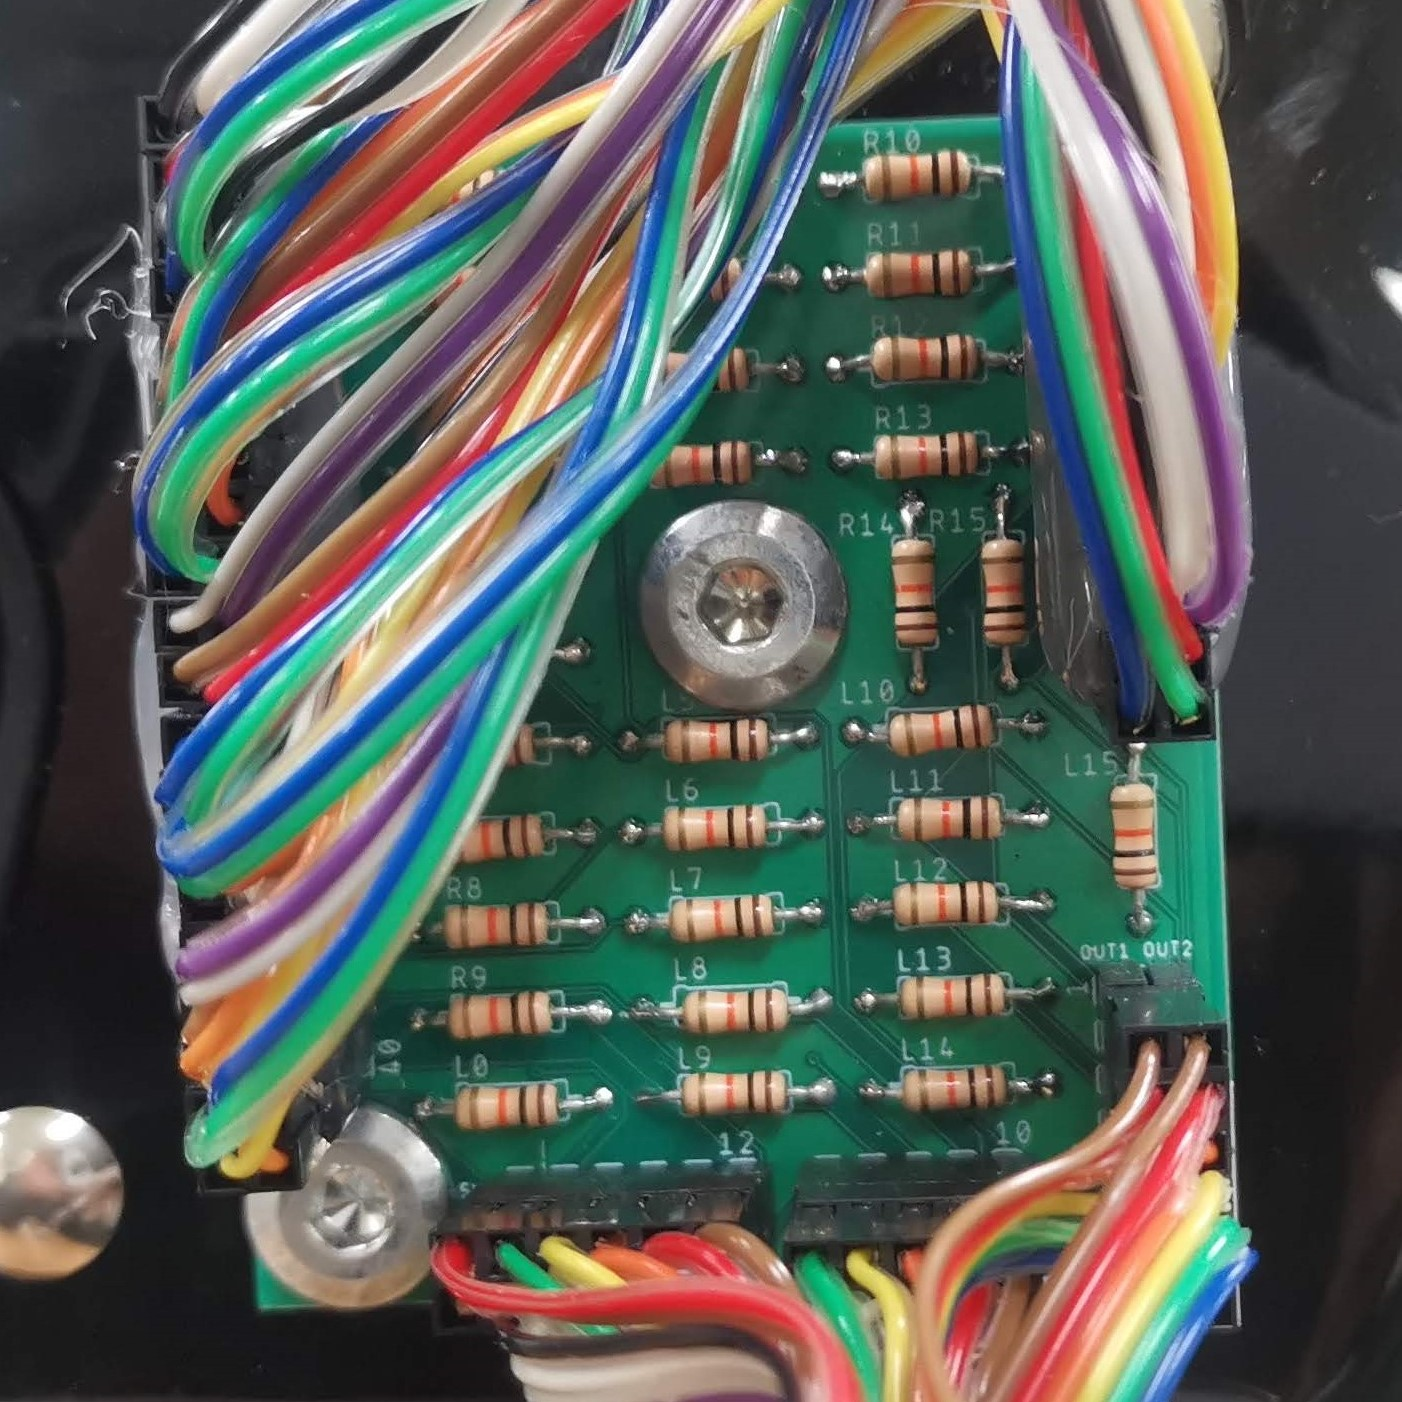
\includegraphics[width=0.6\linewidth]{figure/print.eps}
  \end{center}
  \caption{A printed circuit board connected to 32 pressure sensors}
  \label{fig:print}
\end{figure}




\subsection{User Identification Method}
%In an environment where multiple people are registered in the system and a person wearing a helmet is identified among them, we use the Support Vector Machine (SVM) which is a machine learning algorithm. The SVM is a pattern recognition model using supervised learning that can be applied to classification and regression. In the proposed method, the SVM is trained by the data with the registrant labels in advance. The data of one of the registrants is then entered, and it identifies whom the data is.\par

%複数人がシステムに登録されており,その中からヘルメットを装着した人物を識別する手法では,機械学習アルゴリズムの一つであるSupport Vector Machine(SVM)を用いる.SVMは分類や回帰へ適用できる教師あり学習を用いるパターン認識モデルである.提案手法では登録者でラベル付けしたデータを事前に収集してSVMを学習させておき,その後,登録者のうち1名のデータを入力して登録者を識別する.\par
\subsubsection{Preprocessing}
The data acquisition starts when the user puts on the helmet. The voltage values of all the pressure sensors are almost 5V when the helmet is not worn and the voltage decreases when the helmet is worn. 32 pressure sensors data $\bm{p}(t)=[p_1(t),\cdots,p_{32}(t)]$ are acquired at time $t$ and the system segment the data over 2-second window starting from the $t=T_s$. Time $t=T_s$ is the time when the change of the sum of 32 dimensions per sample $\sum_{i=1}^{32}(p_i(t)-p_i(t-1))$ is first less than 1V for 11 consecutive samples (11/30 second), i.e. $\sum_{i=1}^{32}(p_i(t)-p_i(t-1))<1[V]~(i=T_s,\cdots,T_s-10)$ The average value over the window $x_i(t)=\frac{1}{N}\sum_{t=T_S}^{T_S+N-1}p_i(t)$ for sensor channel $i$ ($i=1,\cdots,32)$ is calculated, where $N$ is the number of samples in the window. We then obtain a 32-dimensional vector $\bm{x}(t)=[x_{1}(t),\dots,p_{32}(t)]$ as a feature. 

% The data acquisition starts when the user puts on the helmet. The voltage values of all the pressure sensors are almost 5V when the helmet is not worn and the voltage decreases when the helmet is worn. 32 pressure sensors data $\bm{p}(t)=[p_1(t),\cdots,p_{32}(t)]$ are acquired at time $t$ and the system segment the data over 2-second window starting from the $t=T_s$, where $T_s$ is the time \textcolor{red}{when the values are stable. **
% More specifically. How do you find the starting point?**}. The average value over the window $x_i(t)=\frac{1}{N}\sum_{t=T_S}^{T_S+N-1}p_i(t)$ for sensor channel $i$ ($i=1,\cdots,32)$ is calculated, where $N$ is the number of samples in the window. We then obtain a 32-dimensional vector $\bm{x}(t)=[x_{1}(t),\dots,p_{32}(t)]$ as a feature. 

\subsubsection{Identification}
Given training data $[\bm{x}_m,y_m]$ $(m=1,\dots, M)$ from the users who are expected to use the helmet by wearing the helmet $M$ times in total in advance, the SVM is trained with the training data, where $y_m$ is the registrant label, such as the registrant's name and number. The input data $\bm{x}_{test}$ collected by the user to be identified is fed into the SVM and the classification result $\hat{y}_{test}$ is obtained.
%**正確に(プログラムできるように)書くこと.被ってない状態から被ったと判定される2秒のウインドウの開始点は厳密にいつ?SVMの詳細は評価のところでよい.パラメータとかカーネルとか.

%データの取得はユーザがヘルメットを装着することで開始する.ヘルメットを装着していない状態ではすべての圧力センサの電圧値がほぼ5Vである.ヘルメットの装着時に圧力センサの電圧値が下降し,値が安定した時刻$t=T_s$[s]から2秒間の32個の圧力センサデータ$p(t)=[p_{0,t},\dots,p_{31,t}]$を取得する.時刻Tとは,1サンプルごとの電圧値の合計の変化量が10サンプル連続で1V以下となった時刻である.この32次元のデータから次元ごとに2秒間に得られたデータの$N$サンプルの平均値$x(t)=\frac{1}{N}\sum_{t=T_S}^{T_S+N-1}p(t)$を計算し,1つの32次元のベクトルを特徴量として得る.事前に$m$回ヘルメットを被って学習データ$[\bm{x}_i,y_i]$ $(i=1,\dots, m)$を収集し,SVMを学習させる.ただし,$y$は登録者ラベル(登録者名や登録者番号など)である.そして,識別したいユーザの入力データ$\bm{x}$をSVMに入力し,識別結果$\hat{y}$を得る.本手法では線形SVMを使用した.

\subsection{User Authentication Method}
\subsubsection{Preprocessing}
In user authentication, 32-dimension pressure sensors data $\bm{p}(t)=[p_1(t),\cdots,p_{32}(t)]$ and its average $\bm{x}(t)=[x_{1}(t),\dots,p_{32}(t)]$ as a feature are obtained in the same manner as in user identification. 

%データの取得は個人識別の場合と同様に,ヘルメットの装着時に圧力センサの電圧値が下降し,値が安定した時刻$t=T_s$[s]から2秒間の32個の圧力センサデータ$p(t)=[p_{0,t},\dots,p_{31,t}]$を取得する.この32次元のデータから次元ごとに2秒間に得られたデータの$N$サンプルの平均値$x(t)=\frac{1}{N}\sum_{t=T_S}^{T_S+N-1}p(t)$を計算し,1つの32次元のベクトルを特徴量として得る.\par

\subsubsection{Similarity calculation}
In user authentication, there are two cases of training data usage: data of a single user is used and data of multiple users is used. 
For single user data, data of only a single user, e.g., owner of the helmet, is registered or data of multiple users are registered but data of one of them whose ID is given is used. For multiple user data, data of multiple users who are expected to use the helmet is used. Given training data $[\bm{x}_m,y_m]$ $(m=1,\dots, M)$ from the user(s) by wearing the helmet $M$ times in advance, the proposed method calculates the Mahalanobis distance, where $y_m$ is the registrant label, such as the registrant's name and number. 

The Mahalanobis distance is one of the methods for calculating the distance between multiple variables, which can be normalized considering the distribution of the data.
The mean vector $\bm{\mu}$ and the variance-covariance matrix $\bm{\Sigma}$ of the training data are calculated by Eqn. \ref{eqn:mu} and \ref{eqn:sigma}.
\begin{eqnarray}
\label{eqn:mu}
  \bm{\mu} &=& \frac{1}{M}\sum_{m=1}^{M}\bm{x}_m \\
\label{eqn:sigma}
  \Sigma_{i,j} &=& \frac{1}{M}\sum_{m=1}^{M}(\bm{x}_i-\bm{\mu})(\bm{x}_j-\bm{\mu})^T
\end{eqnarray}
%分散共分散行列なおしました.iとjの行列よね?

The Mahalanobis distance between training data $\bm{x}_m$ $(m=1,\dots, M)$ and input data $\bm{x}_{test}$ can be calculated with Equation \ref{eqn:mahalanobis}.
\begin{eqnarray}
\label{eqn:mahalanobis}
  d(\bm{x},\bm{x}_m) = \sqrt{(\bm{x}-\bm{x}_m)^{T}\bm{\Sigma}^{-1}(\bm{x}-\bm{x}_m)}
\end{eqnarray}
If the input data are collected from the pre-registered user, the input data $\bm{x}_{input}$ follows the probability distribution of the variance-covariance matrix $\bm{\Sigma}$.
%識別したいユーザの入力データ$\bm{x}$とする.このとき,入力データが事前に登録された本人のデータであれば,入力データ$\bm{x}$と学習データ$\bm{x}_i$は同じ分散共分散行列$\bm{\Sigma}$の確率分布に従うため,入力データ$\bm{x}$と学習データ$\bm{x}_i$のマハラノビス距離は
% \begin{eqnarray}
%   d(\bm{x},\bm{x}_i) = \sqrt{(\bm{x}-\bm{x}_i)^{T}\bm{\Sigma}^{-1}(\bm{x}-\bm{x}_i)}
% \end{eqnarray}
%と定義できる.

%本人認証とは,1人以上の利用者がシステムに登録されており,登録されている人がヘルメットを装着した場合は本人であると認証し,登録されていない人がヘルメットを装着した場合は他人であるとして拒否する手法である.提案手法では,本人認証したい利用者の学習データと未知の装着者の入力データの距離計算方法として,マハラノビス距離を用いる.マハラノビス距離とは多変数間の距離計算手法のひとつであり,データの分布を考慮して正規化した距離を計算できる.\par

%事前に$m$回ヘルメットを被って学習データ$[\bm{x}_i,y_i]$ $(i=1,\dots, m)$を収集する.ただし,$y$は登録者ラベル(登録者名や登録者番号など)である.学習データの平均値ベクトル$\bm{\mu}$と分散共分散行列$\bm{\Sigma}$を次式で求める.

% \begin{eqnarray}
%   \bm{\mu} &=& \frac{1}{m}\sum_{i=1}^{m}\bm{x}_i \\
%   \bm{\Sigma} &=& \frac{1}{m}\sum_{i=1}^{m}(\bm{x}_i-\bm{\mu})(\bm{x}_i-\bm{\mu})^T
% \end{eqnarray}

\subsubsection{Authentication decision}
Let $\theta$ be the threshold value, the user is authenticated if Eqn. \ref{eqn:authentication} is satisfied, while the the user is reejcted if Eqn. \ref{eqn:authentication} is not satisfied.
%, the mean vector $\bm{\mu}$ and the variance-covariance matrix $\bm{\Sigma}$ of each is computed in the same way. It computes the Mahalanobis distance between the input data and each registrant's data set. Then, if Equation \ref{eqn:authentication} is satisfied at least once, it is authenticated, and if it is not satisfied at least once, it is rejected.
\begin{equation}
\label{eqn:authentication}
  \theta \geq \min_m(d(\bm{x}_{input},\bm{x}_m))~(m=1,\cdots,M)
\end{equation}

%閾値を$\theta$とおき,
% \begin{equation}
% \label{eqn:authentication}
%   \theta \geq min_i(d(\bm{x},\bm{x}_i))~(i=1,\dots,m)
% \end{equation}
%を満たす場合,入力データ$\bm{x}$は登録されているいずれかの所有者から得られたデータであると判定し認証する.式\ref{eqn:authentication}を満たさない場合,入力データ$\bm{x}$は登録されているいずれの所有者でもない人物のデータであると判定し拒否する.利用者が複数人登録されている場合は,同様の手順でそれぞれの平均値ベクトル$\bm{\mu}$と分散共分散行列$\bm{\Sigma}$を計算しておく.入力データと登録者一人一人のデータ群とのマハラノビス距離を計算し,一度でも式\ref{eqn:authentication}を満たした場合は認証し,一度も満たさない場合は拒否する.

\subsection{Software}
The program of Arduino MEGA was implemented by Arduino IDE. A computer program that receives data from Arduino MEGA and saves it in csv format was implemented by Python. A computer program to analyze the data was implemented by Python.\par

%Arduino MEGAのプログラムはArduino IDEで実装した.Arduino MEGAからのデータを受信してcsv形式で保存するコンピュータのプログラムはPythonで実装した.保存したデータの解析プログラムはPythonで実装した.\par

In the user identification, the system loads the pre-collected sensor data in csv format. For SVM, \texttt{sklearn.svm.SVC} of a scikit-learn\cite{scikit-learn} library which is an implementation of the standard soft margin SVM is used. We also used \texttt{sklearn.model\_selection.} \texttt{cross\_val\_score} for cross-validation and \texttt{sklearn.model\_selec}\\\texttt{tion.GridSearchCV} for grid search were used for evaluation.\par

%個人識別では,事前に収集したセンサデータのcsvファイルを読み出し,sklearn.svm.SVCを用いて学習と識別を行う.sklearn.svm.SVCとは標準的なソフトマージンSVMを実装したscikit-learn\cite{scikit-learn}のライブラリである.また,評価のために交差検証を行うライブラリであるsklearn.model\_selection.cross\_val\_score\textcolor{blue}{および,グリッドサーチを行うライブラリであるsklearn.model\_selection.GridSearchCV}を使用した.\par

In the user authentication, the system loads pre-collected sensor data in csv format and computes the variance-covariance matrix using \texttt{scipy.spatial.distance}. For the calculation of the Mahalanobis distance, \texttt{sklearn.covariance.MinCovDet} is used for variance-covariance matrix. Minimum Covariance Determinant (MCD) is an algorithm that is robust to outlier values for estimating a variance-covariance matrix. \texttt{sklearn.covariance.MinCovDet} is a scikit-learn library that is implemented Fast-MCD\cite{fast_mcd} which is a faster version of MCD. \texttt{scipy.spatial.distance} is a SciPy\cite{scipy} library that is implemented functions for calculating various distance.

%本人認証では,事前に収集したセンサデータのcsvファイルを読み出し,sklearn.covariance.MinCovDetを用いて分散共分散行列を計算する.分散共分散行列の逆行列から,scipy.spatial.distanceを用いてすべての学習データ$\bm{x}_i$に対する入力データ$\bm{x}$のマハラノビス距離を計算する.sklearn.covariance.MinCovDetとは,異常値に対して頑健な分散共分散行列の推定アルゴリズムであるMinimum Covariance Determinant(MCD)を高速化したFast-MCD\cite{fast_mcd}を実装したscikit-learnのライブラリである.また,scipy.spatial.distanceとは,さまざまな距離計算の関数を実装したSciPy\cite{scipy}のライブラリである.

\section{Evaluation}
\label{sec:evaluation}
This section describes the experiments we conducted to evaluate the effectiveness of the proposed method.
%本節では,提案手法の有効性を評価するために行った実験について説明する.

\subsection{Data Collection}
We asked nine subjects (A$\sim$I, all males, mean age 23 years) to wear the helmet implemented in Section \ref{sec:method} and collected sensor data. The sampling rate is approximately 30 Hz. The subjects put it on for two seconds to collect data, then put it off, and put it on again for two seconds to collect data, tough which a set of two samples is obtained. By collecting data of ten sets (20 samples) from each subject, a total of 180 samples (2 seconds$\times$20 samples$\times$9 subjects) were collected. Up to four sets of data were collected per person per day. In order to collect data on the various positions of the sensors and head as the helmet was worn, a rest period of at least 30 minutes was provided between sets. 
% \textcolor{red}{**Use a figure showing the senor position.**}

%被験者9名(A$\sim$I,全員男性,平均年齢23歳)に\ref{method}節で実装したヘルメットを装着させ,サンプリングレート約30Hzでセンサデータを収集した.2秒間装着してデータを採取し,取り外して再び2秒間装着してデータを採取する試行を1セット(2サンプル)として,日を変えて10セット,合計で2秒$\times$20サンプル$\times$9人のデータを収集した.ヘルメットの装着具合の変化にともなうセンサと頭部のさまざまな位置関係のデータを収集するために,セット間に30分以上の休憩時間を設けた.また,データの収集は1人あたり1日最大4セットとした.

\subsection{User Identification Method}
\subsubsection{Evaluation environment}
We evaluated the proposed method in five-fold cross-validation manner that 80\% (16 samples) of data collected from each subject were trained and 20\% (four samples) were tested. In order to investigate the effect of the number of sensors used, identification accuracies for all combinations of sensors from one sensor to 32 sensors were measured.\par

%収集したデータに対して,各被験者のデータの80\%(16サンプル)を学習させ,20\%(4サンプル)をテストデータとする5分割交差検証によって評価した.使用するセンサの個数による影響も調査するため,1個使用する場合から32個使用する場合までのすべてのセンサの組合せにおいて前述の試行を行った.\par

To simulate a half helmet which is commonly used at a construction site, all combinations of sensors from 1 to 20 sensors aligned in the top half out of 32 sensors; four sensors at the top of the head and 16 sensors around the top half of the head. These 20 sensors are the sensors \#0--\#19 in \figref{position}. In this evaluation, two types of sensor configurations are tested: a full-face helmet with 32 sensors and a half helmet when 20 sensors.

%また,工事現場などで使用されるハーフ型ヘルメットを想定し,32個のセンサのうち頭頂部の4個と頭頂部周囲の16個の合計20個のセンサに限定して,同様に1個使用する場合から20個使用する場合までの全てのセンサの組合せにおいて評価した.この20個とは,\figref{position}のセンサ0~19である.本評価では,32個のセンサを使用する場合をフルフェイス型ヘルメット,20個のセンサを使用する場合をハーフ型ヘルメットと呼ぶ.


\subsubsection{Results and discussion}
The accuracy of user identification with a full-face helmets and a half helmet is shown in \tabref{full_num} and \tabref{half_num}. The numbers shown in ``Sensors used'' are the sensor number in \figref{position}.
For a full-face helmet, when the number of sensors is 32, the number of sensor combination is one ($_{32}C_{32}=1)$, and when the number of sensors is 31, the highest accuracy of  $_{32}C_{31}=32$ combinations is shown in the table. For a half helmet, when the number of sensors is 20, the number of sensor combination is one and when the number of sensor is 19, the highest accuracy of 19 combination is shown in the table. For one through four sensors, the 
regularization parameter of SVM is set to $C=1.0$, and the sensor combination with the highest accuracy was recorded. Then, the best $C$ was searched by grid search for the sensor combination, and the highest accuracy is shown in the tables.

%ここで,"Using Sensors"で示される数字は,図\figref{position}のセンサ番号である.

\begin{table}[!t]
\centering
  \begin{tabular}{cc}

  \begin{minipage}[c]{.45\linewidth}
  \centering
  \caption{Identification accuracy with a full-face helmet; sensors are reduced from 32 to 1.}
  \begin{tabular}{l|c} \hline\hline
    Sensors used & Accuracy \\ \hline
    All & 1.000 \\
    Exclude 1 & 1.000 \\
    \vdots & \vdots \\
    0, 3, 5, 16, 17 & 1.000 \\
    0, 3, 5, 16     & 0.994 \\
    3, 11, 24       & 0.972 \\
    3, 25           & 0.922 \\
    10              & 0.617 \\ \hline
  \end{tabular}
  \label{tab:full_num}
  \end{minipage}&
  \begin{minipage}[c]{.45\linewidth}
  \centering
  \caption{Identification accuracy with a half helmet; sensors are reduced from 20 to 1.}
  \begin{tabular}{l|c} \hline\hline
    Sensors used & Accuracy \\ \hline
    All & 1.000 \\
    Exclude 1 & 1.000 \\
    \vdots & \vdots \\
    0, 3, 5, 16, 17 & 1.000 \\
    0, 3, 5, 16     & 0.994 \\
    0, 3, 13        & 0.983 \\
    3, 16           & 0.928 \\
    10              & 0.617 \\ \hline
  \end{tabular}
  \label{tab:half_num}
  \end{minipage}
  
  \end{tabular}
\end{table}

We found that all the accuracies when 32 and 31 sensors for full-face helmet are used and 20 and 19 sensors for half helmet are used were all 1.000. Therefore, we measured the accuracy from one sensor until the accuracy reaches to 1.000 and skipped the measurement of accuracies for more sensors.\par

%フルフェイス型ヘルメットでの個人識別の精度を\tabref{full_num}に示す.センサ数が32個の場合は,32個すべてを使用する1通りでの精度であり,センサ数が31個の場合は,32個のうち31個を使用する$_{32}C_{31}=$32通りの中で最も高かった精度である.ここで,センサ数が32個および31個の場合の精度を評価したところ1.00であったため,センサ数を1個から増やしていき,精度が1.00に到達するところまでを評価した.\par

For full-face helmet, nine subjects were identified with 100\% accuracy when the number of sensors was five. The accuracy was 99.4\% with four sensors, 97.2\% with three sensors, and 92.2\% with two sensors. However, the accuracy dropped significantly to 61.7\% when the number of sensors was one. 
\par

%結果より,センサ数が5個のとき,9人の識別に100\%の精度で成功した.センサ数が4個で99.4\%,3個で97.2\%,2個で92.2\%と高い精度が得られたが,センサ数が1個では60\%と大幅に下がった.このとき,センサ数が5個以下のそれぞれの個数で精度が最も高かったセンサの組み合わせを記録しておき,さらにその組み合わせにおいてグリッドサーチでパラメータを探索した上で結果としている.\par

%We evaluated the accuracy with 20 or 19 sensors and found that it was 1.00. Therefore, the number of sensors was increased from one, and the accuracy was evaluated until it reached 1.00 as well as the environment in a full-face helmet.\par

%ハーフ型ヘルメットでの個人識別の精度を\tabref{half_num}に示す.この結果もフルフェイス型ヘルメットと同様にセンサ数が20個および19個の場合の精度を評価したところ1.00であったため,センサ数を1個から増やしていき,精度が1.00に到達するところまで評価した.\par

For half helmet, nine subjects were identified with 100\% accuracy when the number of sensors was fine. The accuracy was 99.4\% with four sensors, 98.3\% with three sensors, and 92.8\% with two sensors. However, the accuracy dropped significantly to 61.7\% when the number of sensors was one.\par

%結果より,センサ数が5個のとき,9人の識別に100\%の精度で成功した.センサ数が4個,3個,2個の場合では99.4\%,96.7\%,90.0\%と高い精度が得られたが,センサ数が1個では60\%と大幅に下がった.この結果も同様に,センサ数が5個以下で個数ごとの精度が最も高くなる組み合わせにおいて,さらにグリッドサーチでパラメータを探索して得られた値である.


% \begin{table}[!t]
%   \centering
%   \caption{Personal identification accuracy when the number of sensors on a full-face helmet is reduced from 32 to 1}
%   \begin{tabular}{c|c} \hline\hline
%     Sensor Number & Accuracy \\ \hline
%     32 & 1.000 \\
%     31 & 1.000 \\
%     \vdots & \vdots \\
%     5 & 1.000 \\
%     4 & 0.994 \\
%     3 & 0.972 \\
%     2 & 0.922 \\
%     1 & 0.600 \\ \hline
%   \end{tabular}
%   \label{tab:full_num}
% \end{table}



% \begin{table}[!t]
%   \centering
%   \caption{Personal identification accuracy when the number of sensors on a half helmet is reduced from 20 to 1}
%   \begin{tabular}{c|c} \hline\hline
%     Sensor Number & Accuracy \\ \hline
%     20 & 1.000 \\
%     19 & 1.000 \\
%     \vdots & \vdots \\
%     5 & 1.000 \\
%     4 & 0.994 \\
%     3 & 0.967 \\
%     2 & 0.900 \\
%     1 & 0.600 \\ \hline
%   \end{tabular}
%   \label{tab:half_num}
% \end{table}

Both of the full-face helmet and the half-helmet achieved 100\% accuracy with at least five sensors for the data set used in this experiment. However, the number of sensors required to achieve high accuracy may increases as the number of registrants increases. Focusing on the sensors used for full-face helmet, most of the sensors are less than \#20, which means that sensors in the top half were significant. Sensors not used in half helmet were aligned around neck and ear and the position of the sensors related to the user's head are supposed to be inconsistent. 
%\textcolor{blue}{If we look at 'Using Sensors', sensors '0' and '3' is used in many combinations, and these sensors have a significant impact on the accuracy. In addition, the half-helmets with a limited number of sensors was higher accuracy than the full-face helmets in some cases. In this evaluation, we recorded the combination that has the highest accuracy when the parameter is fixed at C=1.0, and we performed a grid search for the combination. However, even higher accuracy may be achieved by performing a grid search for all combinations.}

% \textcolor{red}{**show which sensor showed the best accuracy in the table and discuss.**}

%これらの結果より,本実験で使用したデータセットに対して,フルフェイス型ヘルメットおよびハーフ型ヘルメットのどちらにおいても,センサ数5個で100\%の精度で識別できることを確認した.しかしながら,登録者数が増加した場合,高い精度を得るためには必要となるセンサ数が増加すると考えられる.
% 'Using Sensors'に注目すると,多くの組み合わせにおいてセンサ'0'と'3'が使用されていることから,これらのセンサが精度に大きく影響していると考えられる.また,フルフェイス型ヘルメットよりも,センサ数を制限しているハーフ型ヘルメットの方が精度が高い場合があった.今回,パラメータをC=1.0で固定した時に最も精度が高くなる組み合わせを記録した上で,その組み合わせにおいてグリッドサーチを行った.しかし,すべての組み合わせについてグリッドサーチを行うことで,さらに高い精度が得られる可能性がある.


\subsection{User Authentication Method}
\subsubsection{Evaluation environment}
One subject was considered to be the individual to be authenticated, i.e. owner, and the remaining eight subjects were considered to be strangers. The authentication accuracy of the owner was measured in 5-fold cross-validation manner; 80\%(16 samples) of the owner's data were registered as training data, and the remaining 20\%(4 samples) data were used as test data. In addition, the authentication accuracy for the strangers were measured using data from all eight strangers (160 samples). All 160 samples were tested in each fold of the cross-validation. All nine subjects were evaluated on a rotation basis.\par

%収集したデータのうち,1名の被験者を本人,残り8名の被験者を他人として,本人としたデータの80\%(16サンプル)を学習データとして登録し,残り20\%(4サンプル)をテストデータとして5分割交差検証を行い本人の認証精度を計測した.さらに,交差検証で使用した5パターンの学習データに対して,他人とした8名すべてのデータ(160サンプル)を用いて他人の認証精度を計測した.また,本人を9名全員ローテーションして評価した.\par

In user authentication, FRR, FAR, and EER are used as indicators of authentication accuracy. FRR is false reject rate at which a registered person is mistakenly considered to be a stranger and rejected. FAR is false accept rate at which a stranger is mistakenly considered to be a registered person and authenticated. The smaller the threshold value $\theta$ in Eqn. \ref{eqn:authentication} is set, the stricter the authentication decision becomes, resulting in increasing FRR. On the other hand, the larger the threshold value $\theta$ is set, the looser the authentication decision becomes, resulting in increasing FAR. 
There is a trade-off between FRR and FAR, and the value at which FRR and FAR become equal is called EER (equal error rate). Normally, the value of EER is used as an indicator to evaluate the performance of authentication methods, and the smaller EER, the better the performance.

%認証精度の評価指標として,FRR,FAR,EERを用いる.FRR(False Reject Rate:本人拒否率)は本人を他人であると誤って判断し拒否する割合である.FAR(False Accept Rate:他人受入率)は他人を本人であると誤って判断し認証する割合である.認証するか否かを決定する閾値を小さく設定するほど認証判定が厳密になるためFRRが増加し,対して閾値を大きく設定するほど認証判定が緩くなるためFARが増加する.FRRとFARはトレードオフの関係にあり,FRRとFARが同値になるときの値をEER(Equal Error Rate:等誤り率)と呼ぶ.通常,本人認証手法の性能評価においてはEERの値が指標として用いられ,EERが小さいほど性能が良いとされる.

\subsubsection{Results and discussion}
EER of each subject is shown in \tabref{EER_num}. ``Average'' means the average EER of all subjects. FRR and FAR for each subject with varying thresholds from 0 to 60 by 1 are shown in \figref{EER}. EER of subjects A, E, G, and I was roughly less than 0.01, which means that the owner fails in authentication less than once a 100 times, and that the strangers break the authentication less than once a 100 times. EER of 0.0097 for user authentication using ear acoustics was reported in Ref. \cite{ear_auth}, therefore, our method achieved comparable performance for four of nine subjects. 

% EER of 0.012 for face authentication was reported in Ref. \cite{face_auth}, therefore, comparable performance was achieved in these subjects.
% \textcolor{red}{More recent paper should be cited.}

\begin{table}[!t]
  \centering
  \caption{EER for the subjects in user authentication.}
  \begin{tabular}{c|c} \hline\hline
    Subject & EER \\ \hline
    A & 0.002 \\
    B & 0.095 \\
    C & 0.050 \\
    D & 0.055 \\
    E & 0.006 \\
    F & 0.094 \\
    G & 0.012 \\
    H & 0.050 \\
    I & 0.000 \\ \hline
    Average & 0.076 \\ \hline
  \end{tabular}
  \label{tab:EER_num}
\end{table}


% For subject E, FRR and FAR crossed at a threshold of approximately 60, which is greater than the other subjects. 
% This is because there were outliers in the collected pressure data samples, and it was necessary to increase the threshold value to authenticate the outliers correctly. \textcolor{red}{How many outliers? Please visualize. Explain more precisely, why FAR is very small?}\par

%各被験者のEERを\tabref{EER_num}に示す.また,閾値を変化させたときの各被験者のFRRとFARを\figref{EER}に示す.Totalは被験者全員の平均を示している.\tabref{EER_num}より被験者A,E,G,IのEERはおおよそ0.01以下と良い結果が得られた.これは,検証に用いたデータセットにおいて,本人は100回に1回以下の割合で認証に失敗し,他人は100回に1回以下の割合で認証を突破することを意味している.文献\cite{ear_auth}において,耳の音響特性を使用した認証のEERが0.97%であると報告されていることを考慮すると,これらの被験者については同等の性能が得られたといえる.
%文献\cite{face_auth}において,顔認証のEERが0.012であると報告されていることを考慮すると,これらの被験者については同等の性能が得られたといえる.

%これは収集した圧力データのサンプルに外れ値が存在したため,外れ値を正しく認証するために閾値を大きくする必要があったためである.\par


\begin{figure}[!t]
  \centering
    \includegraphics[width=1\linewidth]{figure/EER.eps}
  \caption{FRR and FAR for the subjects in user authentication.}
  \label{fig:EER}
\end{figure}

The next most accurate subjects are C, D, and H, with EER of approximately 0.05. In order to determine the cause of the decline in accuracy compared with subject A, E, G, I, all collected data were compressed to the first principal component and the second principal component by principal component analysis (PCA). The results of this data plotted on a two-dimensional plane are shown in \figref{PCA}. Looking at the plots of subject C, one sample of data of subject C is close to data of subject I and the variance in the first principal component is large, which would deteriorate the accuracy. On the other hand, the data for subjects D and H overlapped each other significantly, which affected the accuracy of the both subjects.\par

%次に精度が良い被験者はC,D,Hであり,EERはおおよそ0.05である.ここで精度の低下の要因を究明するために,収集したすべてのデータに対して主成分分析を行い,第一主成分および第二主成分の2次元に圧縮したデータを2次元平面上にプロットし,目視で確認した.結果を\figref{PCA}に示す.\figref{PCA}より,被験者Cについて見ると,被験者Cのデータ群のうち1サンプルが被験者Iのデータ群と近い位置にあるが,他の被験者のデータ群との重なりは見られない.しかしながら,第一主成分方向の分散が大きい.一方,被験者D,Hのデータ群は互いに大きく重なっており,両者が影響し合って精度が低下したと考えられる.\par

\begin{figure}[!t]
  \centering
    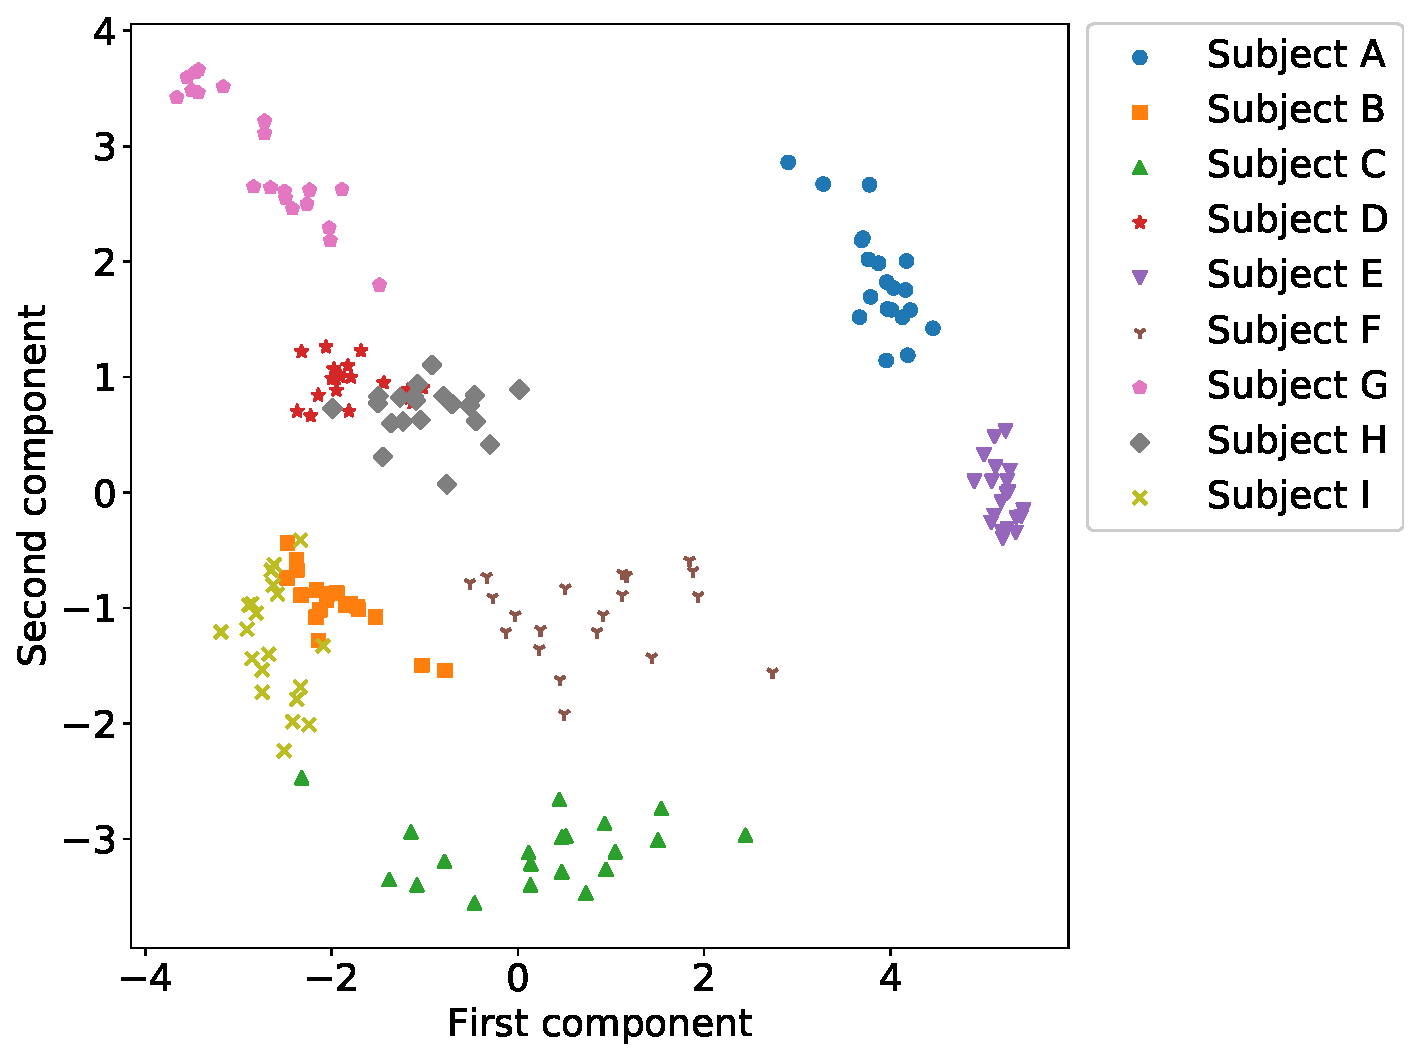
\includegraphics[width=1\linewidth]{figure/PCA.eps}
  \caption{Principal component distribution of 32-dimensional features compressed into two dimensions by PCA}
  \label{fig:PCA}
\end{figure}

The least accurate subjects are B and F, with EER of approximately 0.095. Data of subject B has a small variance and there is some overlap with data of subject I. However, EER of subject I was 0, which is perfect authentication. Therefore, the overlap of these data groups is likely due to the loss of data when they are compressed into two dimensions by principal component analysis. 

On the other hand, subject F's data does not show any overlap with the other subjects' data, but there is a large variance to both directions for the first and second principal components. Considering the effect of data compression by PCA, duplication with other subjects' data groups can be inferred in the 32-dimensional data. The accuracy of subjects B and C, who has data groups located close to subject F's data groups, may have been affected by the scattered data of subject F. In particular, the accuracy of subject B is likely to be lower than that of subject C because the two samples of subject B are located in close proximity to subject F's data group.\par

%最も精度が悪かった被験者はB,Fであり,これらの被験者のEERはおおよそ0.095であった.被験者Bのデータ群は分散が小さいが,被験者Iのデータ群との重なりが見られる.しかしながら,検証に用いたデータセットにおける被験者IのEERは0であり,誤りなく判別ができていた.したがって,これらのデータ群の重なりは主成分分析で2次元に圧縮した際のデータの損失による影響だと考えられる.一方,被験者Fのデータ群は他の被験者のデータ群との重なりが見られないが,第一主成分と第二主成分の両方向の分散が大きい.主成分分析によるデータ圧縮の影響を考慮すると,32次元のデータでは他の被験者のデータ群との重複が推察される.被験者Fのデータの散らばりに影響されて,被験者Fのデータ群の近くに位置する被験者B,Cの精度も低下したと考えられる.特に,被験者Bは2サンプルが被験者Fのデータ群と近い位置に存在するため,被験者Cに比べて精度が低下したと考えられる.\par

Data of subject E are located at the rightmost points. In addition, the variance is small so the data are considered to be very distinctive. For subject E in \figref{EER}, FRR and FAR crossed at a threshold of approximately 60, which is greater than the other subjects. This is because the data are quite different from the others and the FAR did not increase by increasing the threshold.\par

%被験者Eのデータ群は最も右端に位置する.また,分散が小さく,データが非常に特徴的であると考えられる.\figref{EER}より,被験者Eについては,閾値が他の被験者よりも大きい60程度でFRRとFARが交差している.これはデータが特徴的で,閾値を大きくしてもFARが増加しなかったからである.\par

Summarizing the results of user authentication, the mean EER of all subjects was approximately 0.076. It is necessary to validate with data from a larger number of subjects because there was a difference in EER between subjects. 
%The proposed method uses the distance between the training data and the input data for authentication, so that the accuracy is expected to be improved by increasing the number of training data. 
In addition, we will also examine a method for authentication using time series pressure data of helmet from start wearing to finish wearing.

%被験者全員の平均EERは約0.076であった.被験者ごとのEERに差が見られたことから,より多くの被験者のデータを用いて検証する必要がある.また,提案手法は学習データと入力データの距離を用いて認証を行うため,学習データ数をさらに増やすことで精度の改善が見込まれる.このほか,ヘルメットを装着する一連の流れにおける時系列圧力データを用いて認証する手法についても今後検証する.

\section{Conclusion}
\label{sec:conclusion}
In this study, we proposed a method to identify individuals based on individual differences in head shapes which is measured by wearing a helmet with pressure sensors. We implemented the prototype device and evaluated the proposed method. The prototype device is a commercially available full-face helmet and we attached 32 pressure sensors inside the helmet. In the evaluation, we obtained the sensor values for 2 seconds 20 times from nine subjects as head shape data. Using the acquired data, we evaluated the accuracy of user identification to determine who is wearing the helmet among the registrants and the accuracy of user authentication to determine whether the helmet wearer is the registrant or not.\par

%本研究では,圧力センサを内部に取り付けたヘルメットを装着することで頭部の形状を計測して,頭部形状の個人差から個人を識別する手法を提案し,プロトタイプデバイスの実装と評価を行った.プロトタイプデバイスは市販のフルフェイス型ヘルメットを加工し,圧力センサを取り付けた.評価では,プロトタイプデバイスからデータを取得するためにデータ収集プログラムを作成し,頭部形状データとして被験者9人からそれぞれ2秒間のセンサ値を20回分取得した.複数の登録者のうち誰が装着したのかを判別することを目的とした個人識別と,二輪車の鍵のように用いることを想定して1名の登録者であるか他人であるかを判別することを目的とする本人認証を行った.\par

Since the accuracy was 100\% with 32 sensors in the user identification, we tested how the accuracy changed by decreasing the number of sensors. The results showed that the smallest number of sensors showing 100\% accuracy was five. EER of four out of nine subjects showed less than 0.012, and the average EER was 0.076 in the authentication. These results suggest that our method is effective as a user identification method. In the future, we will collect more data and evaluate the proposed method in a real environment.

%評価実験では,個人識別では非常に精度が高かったため,識別に使用するセンサ数を減少させて識別精度がどのように変化するかを検証した.その結果,本実験で使用したデータセットに対して一番効率の良いセンサ数は,フルフェイス型ヘルメットおよび,ハーフ型ヘルメットのどちらの場合も5個であった.本人認証では認証の精度の評価指標であるEERが9名中4名が0.012以下,平均0.076という結果が得られた.これらの結果より,本手法は個人識別手法として有効であると考えられる.今後はさらなるデータの収集を行い,実環境での提案手法の評価を行う.


% \section{Citations and Bibliographies}

% The use of \BibTeX\ for the preparation and formatting of one's
% references is strongly recommended. Authors' names should be complete
% --- use full first names (``Donald E. Knuth'') not initials
% (``D. E. Knuth'') --- and the salient identifying features of a
% reference should be included: title, year, volume, number, pages,
% article DOI, etc.

% The bibliography is included in your source document with these two
% commands, placed just before the \verb|\end{document}| command:
% \begin{verbatim}
%   \bibliographystyle{ACM-Reference-Format}
%   \bibliography{bibfile}
% \end{verbatim}
% where ``\verb|bibfile|'' is the name, without the ``\verb|.bib|''
% suffix, of the \BibTeX\ file.

% Citations and references are numbered by default. A small number of
% ACM publications have citations and references formatted in the
% ``author year'' style; for these exceptions, please include this
% command in the {\bfseries preamble} (before
% ``\verb|\begin{document}|'') of your \LaTeX\ source:
% \begin{verbatim}
%   \citestyle{acmauthoryear}
% \end{verbatim}

%   Some examples.  A paginated journal article \cite{Abril07}, an
%   enumerated journal article \cite{Cohen07}, a reference to an entire
%   issue \cite{JCohen96}, a monograph (whole book) \cite{Kosiur01}, a
%   monograph/whole book in a series (see 2a in spec. document)
%   \cite{Harel79}, a divisible-book such as an anthology or compilation
%   \cite{Editor00} followed by the same example, however we only output
%   the series if the volume number is given \cite{Editor00a} (so
%   Editor00a's series should NOT be present since it has no vol. no.),
%   a chapter in a divisible book \cite{Spector90}, a chapter in a
%   divisible book in a series \cite{Douglass98}, a multi-volume work as
%   book \cite{Knuth97}, an article in a proceedings (of a conference,
%   symposium, workshop for example) (paginated proceedings article)
%   \cite{Andler79}, a proceedings article with all possible elements
%   \cite{Smith10}, an example of an enumerated proceedings article
%   \cite{VanGundy07}, an informally published work \cite{Harel78}, a
%   doctoral dissertation \cite{Clarkson85}, a master's thesis:
%   \cite{anisi03}, an online document / world wide web resource
%   \cite{Thornburg01, Ablamowicz07, Poker06}, a video game (Case 1)
%   \cite{Obama08} and (Case 2) \cite{Novak03} and \cite{Lee05} and
%   (Case 3) a patent \cite{JoeScientist001}, work accepted for
%   publication \cite{rous08}, 'YYYYb'-test for prolific author
%   \cite{SaeediMEJ10} and \cite{SaeediJETC10}. Other cites might
%   contain 'duplicate' DOI and URLs (some SIAM articles)
%   \cite{Kirschmer:2010:AEI:1958016.1958018}. Boris / Barbara Beeton:
%   multi-volume works as books \cite{MR781536} and \cite{MR781537}. A
%   couple of citations with DOIs:
%   \cite{2004:ITE:1009386.1010128,Kirschmer:2010:AEI:1958016.1958018}. Online
%   citations: \cite{TUGInstmem, Thornburg01, CTANacmart}. Artifacts:
%   \cite{R} and \cite{UMassCitations}.

% \section{Acknowledgments}

% Identification of funding sources and other support, and thanks to
% individuals and groups that assisted in the research and the
% preparation of the work should be included in an acknowledgment
% section, which is placed just before the reference section in your
% document.

% This section has a special environment:
% \begin{verbatim}
%   \begin{acks}
%   ...
%   \end{acks}
% \end{verbatim}
% so that the information contained therein can be more easily collected
% during the article metadata extraction phase, and to ensure
% consistency in the spelling of the section heading.

% Authors should not prepare this section as a numbered or unnumbered {\verb|\section|}; please use the ``{\verb|acks|}'' environment.

% \section{Appendices}

% If your work needs an appendix, add it before the
% ``\verb|\end{document}|'' command at the conclusion of your source
% document.

% Start the appendix with the ``\verb|appendix|'' command:
% \begin{verbatim}
%   \appendix
% \end{verbatim}
% and note that in the appendix, sections are lettered, not
% numbered. This document has two appendices, demonstrating the section
% and subsection identification method.

% \section{SIGCHI Extended Abstracts}

% The ``\verb|sigchi-a|'' template style (available only in \LaTeX\ and
% not in Word) produces a landscape-orientation formatted article, with
% a wide left margin. Three environments are available for use with the
% ``\verb|sigchi-a|'' template style, and produce formatted output in
% the margin:
% \begin{itemize}
% \item {\verb|sidebar|}:  Place formatted text in the margin.
% \item {\verb|marginfigure|}: Place a figure in the margin.
% \item {\verb|margintable|}: Place a table in the margin.
% \end{itemize}

% %%
% %% The acknowledgments section is defined using the "acks" environment
% %% (and NOT an unnumbered section). This ensures the proper
% %% identification of the section in the article metadata, and the
% %% consistent spelling of the heading.
% \begin{acks}
% To Robert, for the bagels and explaining CMYK and color spaces.
% \end{acks}

%%
%% The next two lines define the bibliography style to be used, and
%% the bibliography file.
\bibliographystyle{ACM-Reference-Format}
\bibliography{references}

% %%
% %% If your work has an appendix, this is the place to put it.
% \appendix

% \section{Research Methods}

% \subsection{Part One}

% Lorem ipsum dolor sit amet, consectetur adipiscing elit. Morbi
% malesuada, quam in pulvinar varius, metus nunc fermentum urna, id
% sollicitudin purus odio sit amet enim. Aliquam ullamcorper eu ipsum
% vel mollis. Curabitur quis dictum nisl. Phasellus vel semper risus, et
% lacinia dolor. Integer ultricies commodo sem nec semper.

% \subsection{Part Two}

% Etiam commodo feugiat nisl pulvinar pellentesque. Etiam auctor sodales
% ligula, non varius nibh pulvinar semper. Suspendisse nec lectus non
% ipsum convallis congue hendrerit vitae sapien. Donec at laoreet
% eros. Vivamus non purus placerat, scelerisque diam eu, cursus
% ante. Etiam aliquam tortor auctor efficitur mattis.

% \section{Online Resources}

% Nam id fermentum dui. Suspendisse sagittis tortor a nulla mollis, in
% pulvinar ex pretium. Sed interdum orci quis metus euismod, et sagittis
% enim maximus. Vestibulum gravida massa ut felis suscipit
% congue. Quisque mattis elit a risus ultrices commodo venenatis eget
% dui. Etiam sagittis eleifend elementum.

% Nam interdum magna at lectus dignissim, ac dignissim lorem
% rhoncus. Maecenas eu arcu ac neque placerat aliquam. Nunc pulvinar
% massa et mattis lacinia.

\end{document}
\endinput
%%
%% End of file `sample-authordraft.tex'.
